% !TeX root = main.tex
% Continuacion del informe. Comparte preambulo, estilos y contadores.
\clearpage
\begingroup
\setlength{\emergencystretch}{2em}
\section{Fase 5: Diseño y Descomposición del Monolito}
\label{sec:fase5}
El TP Integrador II continúa el despliegue de BookStack mediante el patrón
\textit{Strangler Fig}. La Fase 5 establece los límites funcionales y sus
contratos de integración. El apartado A1 presenta el inventario del monolito,
la matriz de acoplamiento y el mapa de contextos que sustentan la extracción
por API REST y Webhooks.

\subsection{A1: Análisis del Monolito y Mapa de Contextos}
\label{sec:fase5-a1}
\subsubsection{Método y procedencia de la evidencia}
El relevamiento se ejecutó por SSH como \texttt{arqweb} en
\texttt{arqwebserver}. Se contrastaron el catálogo de MariaDB
\path{information_schema}, la estructura de las tablas y el código PHP de
\path{/var/www/bookstack/app}. La recolección del 11 de noviembre de 2026
conserva 41 tablas, 280 columnas y 479 archivos PHP. Se verificaron las cinco
sumas SHA-256 del paquete recibido y se extrajeron 51 fragmentos de código
con archivo y número de línea para sostener la trazabilidad de los accesos.

El respaldo versionable se conserva en el directorio de evidencias.
\begin{quote}\small
\path{cna/docs/evidencias/fase5/relevamiento/}
\end{quote}
Contiene
\texttt{tablas.tsv}, \texttt{columnas.tsv}, \texttt{claves.tsv} y
\path{codigo-verificado.txt}. El índice de referencias R01--R11 está en
\path{cna/docs/fase5-a1-trazabilidad.md}. La asociación funcional se obtiene
siguiendo consultas, relaciones ORM y llamadas entre módulos, además de
las restricciones declaradas por la base de datos.

La comprobación inicial registró los tres servicios LNMP activos y
\texttt{HTTP/1.1 200 OK} para \texttt{/login}, consultado por HTTPS desde la
VM mediante resolución local del dominio y \texttt{curl -k}
(Figura~\ref{fig:f5-base}).

\begin{figure}[H]
\centering
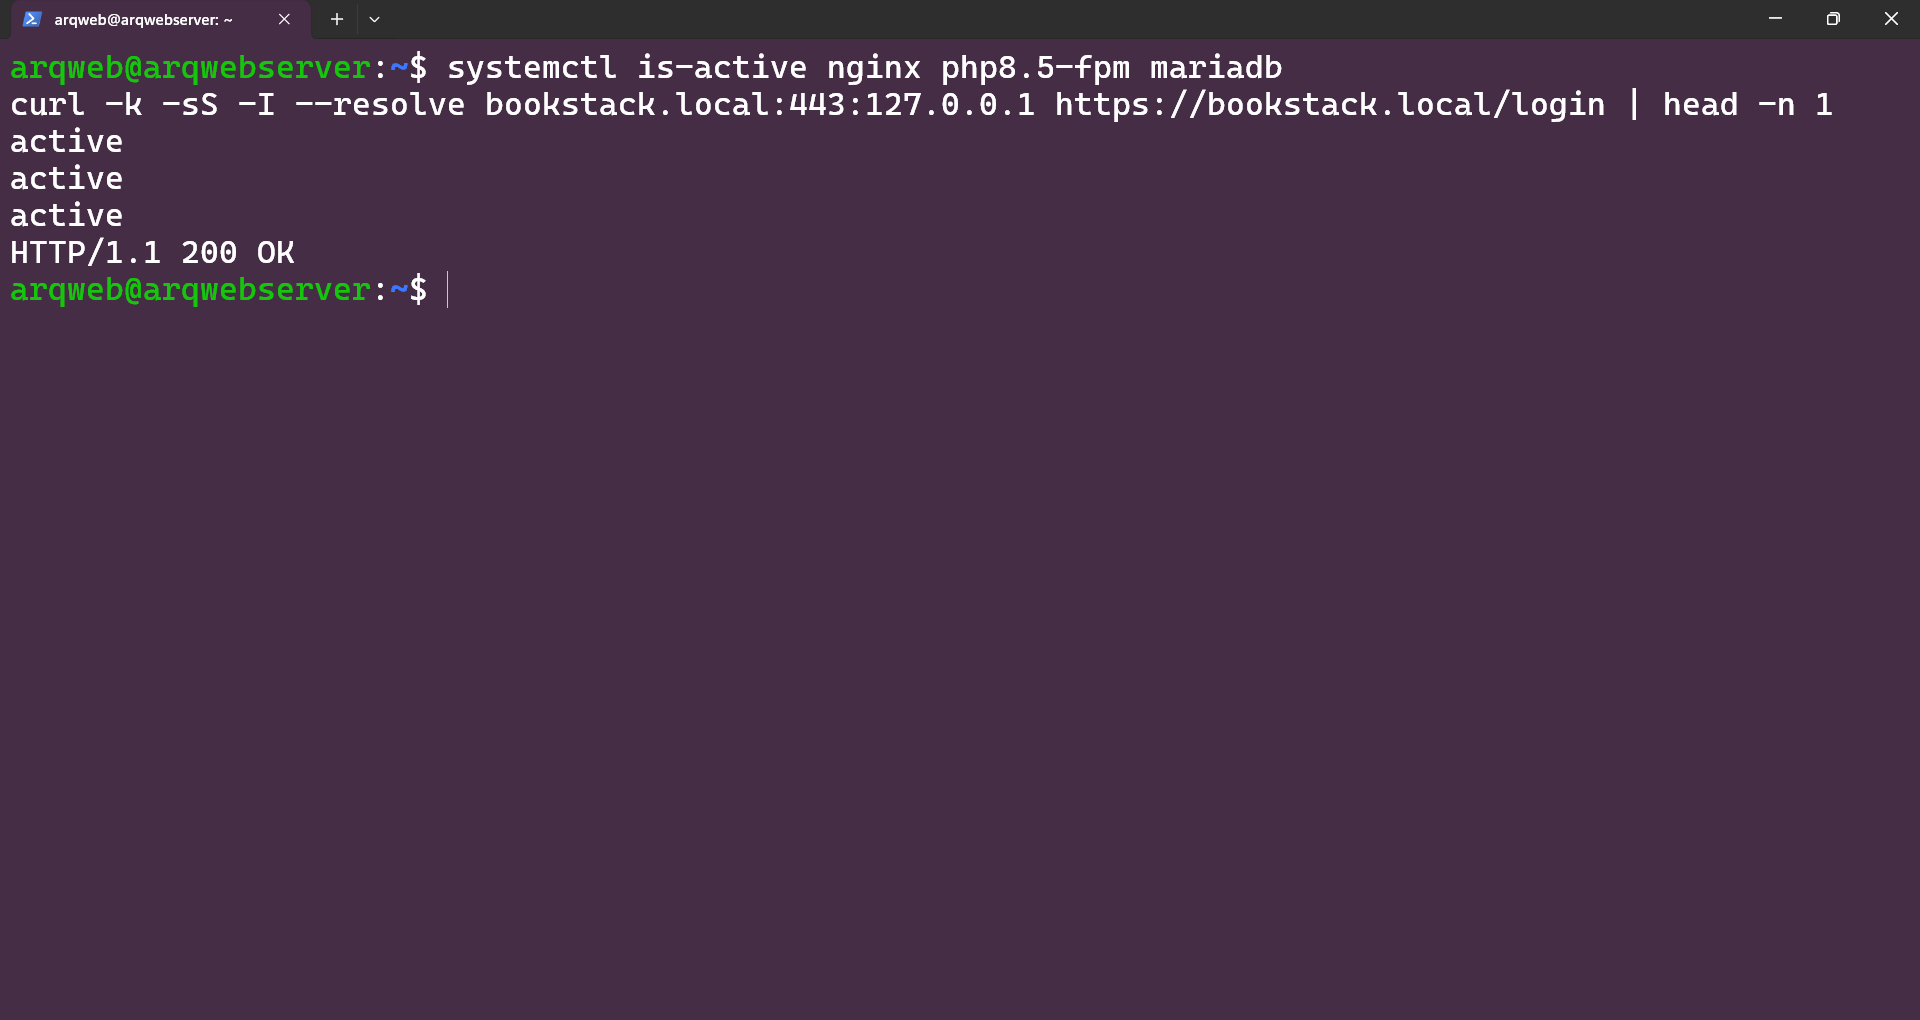
\includegraphics[width=\textwidth,height=0.42\textheight,keepaspectratio]{../../../cna/docs/evidencias/fase5/BASE-01-bookstack-activo.png}
\caption{Continuidad operativa del monolito al iniciar A1. Nginx, PHP-FPM y MariaDB activos y respuesta HTTPS del login.}
\label{fig:f5-base}
\end{figure}

\begin{figure}[H]
\centering
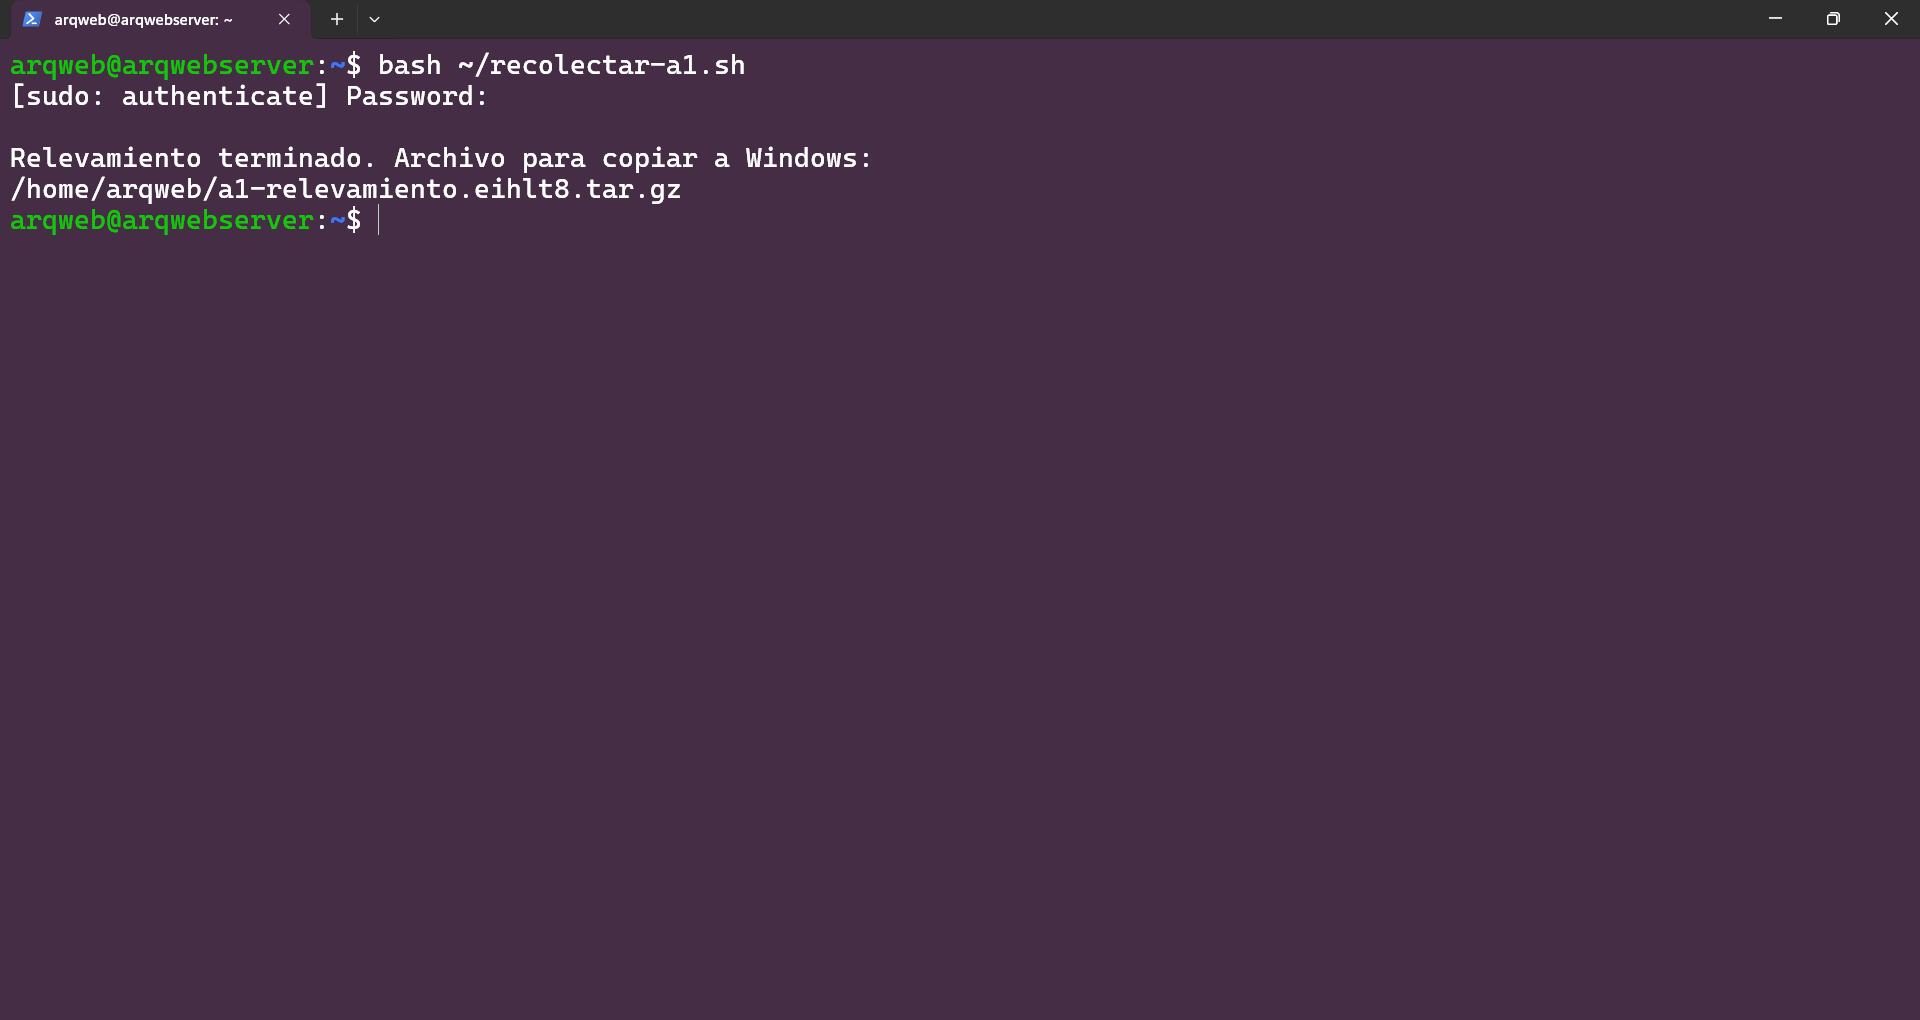
\includegraphics[width=\textwidth,height=0.42\textheight,keepaspectratio]{../../../cna/docs/evidencias/fase5/F5-E1-04-recoleccion-esquema-codigo.png}
\caption{Respaldo de F5-E1. Recolección del esquema y código ejecutada en el nodo; el paquete resultante conserva las fuentes del análisis.}
\label{fig:f5-recoleccion}
\end{figure}

\subsubsection{F5-E1: Inventario del esquema y módulos funcionales}
\label{sec:f5-inventario}
La consulta a \path{information_schema.TABLES} identifica 41 tablas en
\texttt{bookstack\_db} (Figura~\ref{fig:f5-e1-inventario}). El contenido se
organiza en \texttt{entities}, que almacena la identificación, el tipo, el
nombre y las referencias jerárquicas, y en dos tablas de datos específicos.
\path{entity_container_data} almacena atributos de libros, capítulos y
estanterías; \texttt{entity\_page\_data} conserva HTML, texto, Markdown y
estado de las páginas.

La clave de \texttt{entities} combina \texttt{id} y \texttt{type}. La
relación con los datos de contenedores combina ID y tipo, mientras que los
datos de páginas se unen mediante \texttt{page\_id}. Los términos de búsqueda
referencian la entidad por ID y tipo. La actividad utiliza
\texttt{loggable\_id} y \texttt{loggable\_type}, junto con el usuario y las
marcas temporales (Figura~\ref{fig:f5-e1-columnas}).

\begin{figure}[H]
\centering
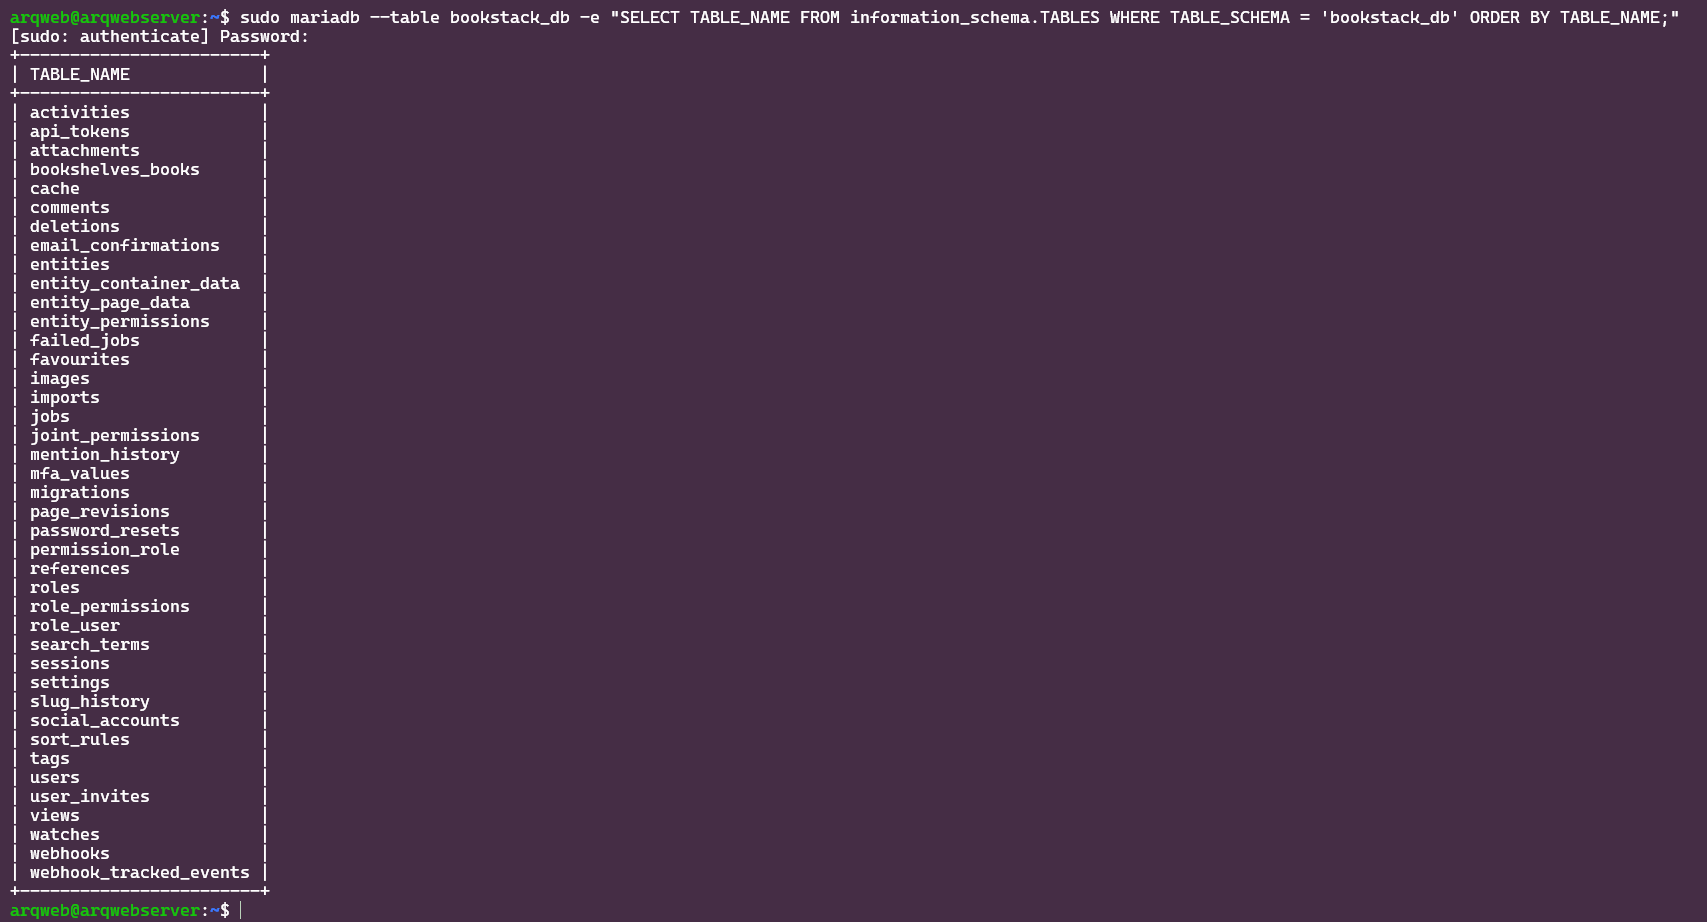
\includegraphics[width=\textwidth,height=0.64\textheight,keepaspectratio]{../../../cna/docs/evidencias/fase5/F5-E1-01-inventario-tablas.png}
\caption{F5-E1. Inventario de las 41 tablas de BookStack mediante el catálogo de MariaDB.}
\label{fig:f5-e1-inventario}
\end{figure}

\begin{figure}[H]
\centering
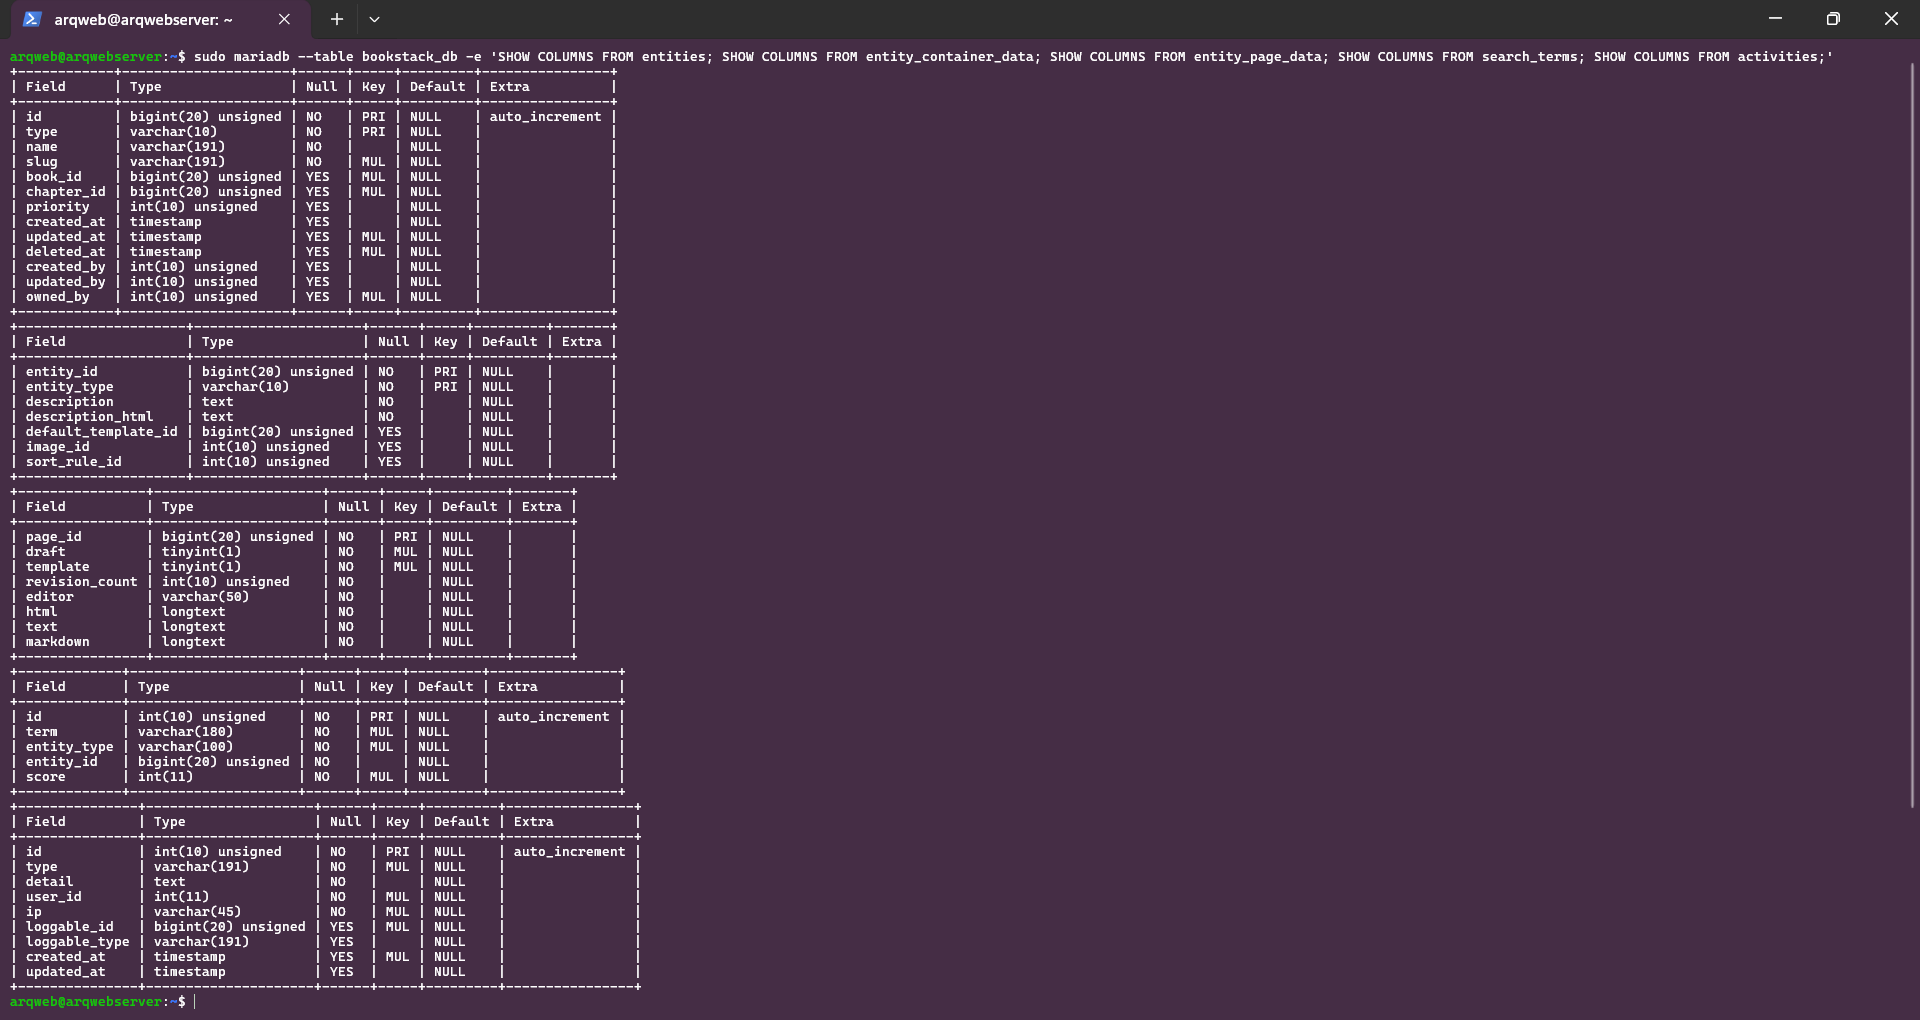
\includegraphics[width=\textwidth,height=0.64\textheight,keepaspectratio]{../../../cna/docs/evidencias/fase5/F5-E1-02-columnas.png}
\caption{F5-E1. Columnas y claves de las tablas de entidades, datos específicos, índice y actividad.}
\label{fig:f5-e1-columnas}
\end{figure}

La consulta de claves foráneas salientes sobre las cinco tablas iniciales
de contenido, índice y actividad devuelve cero filas
(Figura~\ref{fig:f5-e1-fk}). Al ampliar la consulta a todo el esquema aparecen
cuatro restricciones, todas en los pivotes de autorización
(Figura~\ref{fig:f5-e1-fk-roles}). Las relaciones restantes del análisis se
sostienen en las uniones y relaciones del código instalado.

\begin{figure}[H]
\centering
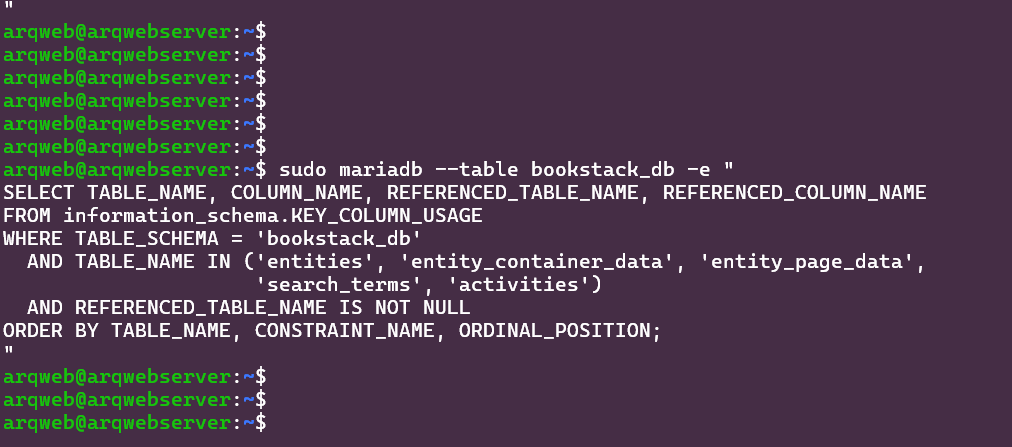
\includegraphics[width=\textwidth,height=0.45\textheight,keepaspectratio]{../../../cna/docs/evidencias/fase5/F5-E1-03-claves-foraneas.png}
\caption{F5-E1. Consulta sin claves foráneas salientes declaradas para las cinco tablas iniciales del relevamiento.}
\label{fig:f5-e1-fk}
\end{figure}

\begin{figure}[H]
\centering
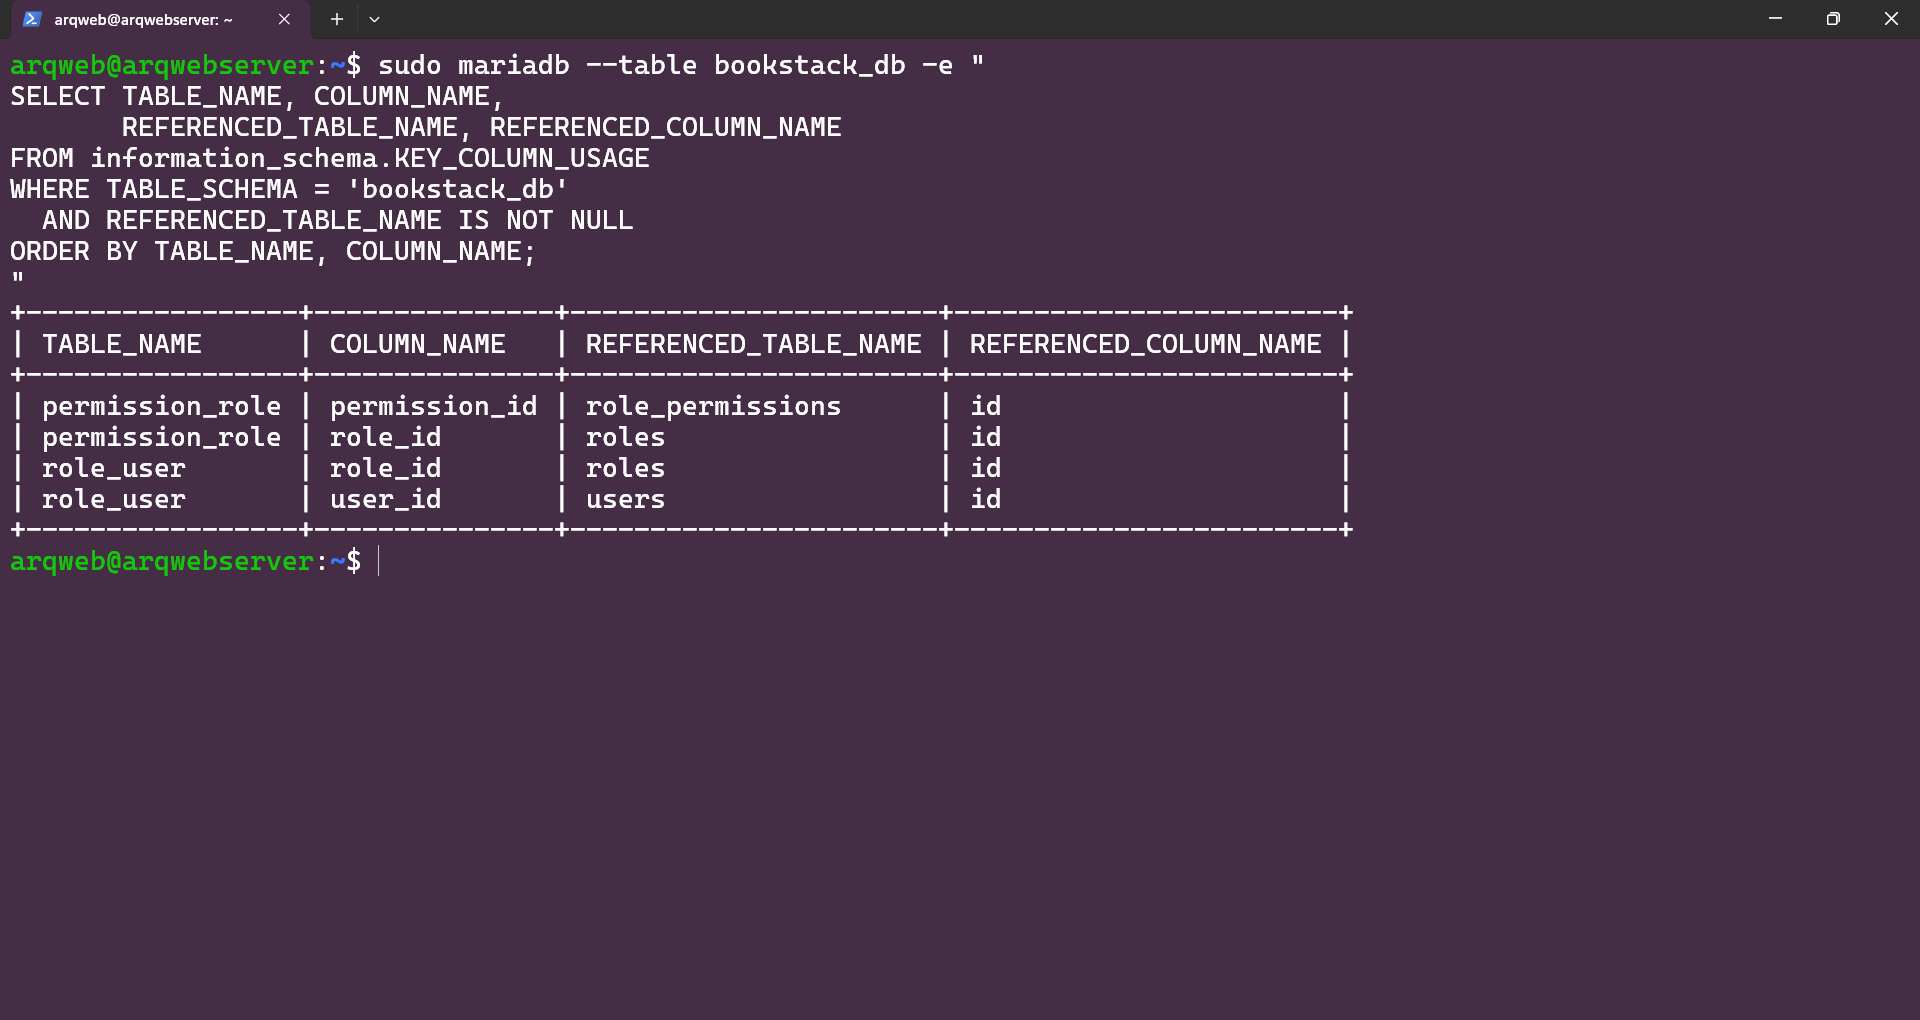
\includegraphics[width=\textwidth,height=0.53\textheight,keepaspectratio]{../../../cna/docs/evidencias/fase5/F5-E1-05-fk-usuarios-roles.png}
\caption{F5-E1. Las cuatro claves foráneas declaradas en el esquema completo relacionan usuarios, roles y permisos.}
\label{fig:f5-e1-fk-roles}
\end{figure}

\begin{table}[H]
\centering\small
\begin{tabularx}{\textwidth}{XX}
\toprule
\textbf{Columna origen} & \textbf{Columna referenciada} \\
\midrule
\path{permission_role.permission_id} & \path{role_permissions.id} \\
\path{permission_role.role_id} & \path{roles.id} \\
\path{role_user.role_id} & \path{roles.id} \\
\path{role_user.user_id} & \path{users.id} \\
\bottomrule
\end{tabularx}
\caption{Restricciones de integridad referencial verificadas en MariaDB.}
\label{tab:f5-fk}
\end{table}

La Tabla~\ref{tab:f5-modulos} identifica los seis módulos funcionales y sus
recorridos principales. Los identificadores de tabla T01--T17 se definen
en la Tabla~\ref{tab:f5-tablas} y se reutilizan en la matriz para conservar
la legibilidad de los nombres y de los accesos.

\begingroup\small
\begin{xltabular}{\textwidth}{p{2.6cm}XX}
\caption{Inventario funcional de los seis módulos, con persistencia y trazabilidad.}\label{tab:f5-modulos}\\
\toprule
\textbf{Módulo} & \textbf{Tablas y dependencias} & \textbf{Recorrido verificado} \\
\midrule\endhead
Contenido & T01--T04, T06 y T07. Delega indexación, actividad y permisos. & Guardado de entidad y datos específicos; revisiones; etiquetas y pivote de estanterías. R01--R03 y R11. \\
Búsqueda & T01--T03, T05 y T06. Consulta visibilidad. & Indexación de nombre, cuerpo y etiquetas; reemplazo de términos y unión por ID y tipo. R04. \\
Actividad / auditoría & T08 y T09; consulta entidades, avatares y permisos efectivos. & Persistencia del registro, carga de actor y objeto y llamada a Webhooks. R05. \\
Exportación & T01--T03; T06, T16 y T17 para ZIP; autorización de contenido. & Controladores, consultas visibles, árbol del libro y formateo Markdown/PDF; archivos de ZIP. R06. \\
Imágenes / adjuntos & T16 y T17; T03 y T04 para limpieza; autorización de la página. & Alta, actualización y baja de archivos y registros; detección de referencias en HTML y revisiones. R07--R08. \\
Usuarios / permisos & T09--T15; referencias de autoría y propiedad en contenido y medios. & Gestión de cuentas y roles; asignación de permisos y reconstrucción de permisos efectivos. R09--R10. \\
\bottomrule
\end{xltabular}
\endgroup

\begin{table}[H]
\centering\small
\begin{tabularx}{\textwidth}{cXc}
\toprule
\textbf{ID} & \textbf{Tabla física} & \textbf{Compartida en la matriz} \\
\midrule

T01 & \path{entities} & Sí \\

T02 & \path{entity_container_data} & Sí \\

T03 & \path{entity_page_data} & Sí \\

T04 & \path{page_revisions} & Sí \\

T05 & \path{search_terms} & Sí \\

T06 & \path{tags} & Sí \\

T07 & \path{bookshelves_books} & Un recorrido \\

T08 & \path{activities} & Sí \\

T09 & \path{users} & Sí \\

T10 & \path{roles} & Un recorrido \\

T11 & \path{role_user} & Un recorrido \\

T12 & \path{role_permissions} & Un recorrido \\

T13 & \path{permission_role} & Un recorrido \\

T14 & \path{entity_permissions} & Un recorrido \\

T15 & \path{joint_permissions} & Sí \\

T16 & \path{images} & Sí \\

T17 & \path{attachments} & Sí \\

\bottomrule
\end{tabularx}
\caption{Tablas principales de A1. Una tabla compartida presenta accesos atribuidos a más de un módulo, incluidos los delegados.}
\label{tab:f5-tablas}
\end{table}

Las otras 24 tablas del catálogo corresponden a funciones auxiliares y
soporte transversal. Su clasificación completa aparece en la
Tabla~\ref{tab:f5-auxiliares}; junto con las 17 tablas principales cubre el
inventario de 41 entradas.

\begin{table}[H]
\centering\small
\begin{tabularx}{\textwidth}{p{3.5cm}X}
\toprule
\textbf{Grupo funcional} & \textbf{Tablas} \\
\midrule
Conversación y seguimiento & \path{comments}, \path{favourites}, \path{mention_history}, \path{views}, \path{watches} \\
Referencias, historial y orden & \path{references}, \path{slug_history}, \path{sort_rules}, \path{deletions} \\
Integraciones y notificaciones & \path{webhooks}, \path{webhook_tracked_events} \\
Acceso e identidad & \path{api_tokens}, \path{email_confirmations}, \path{mfa_values}, \path{password_resets}, \path{sessions}, \path{social_accounts}, \path{user_invites} \\
Importación & \path{imports} \\
Plataforma y configuración & \path{cache}, \path{jobs}, \path{failed_jobs}, \path{migrations}, \path{settings} \\
\bottomrule
\end{tabularx}
\caption{Clasificación funcional de las tablas auxiliares del catálogo.}
\label{tab:f5-auxiliares}
\end{table}

\subsubsection{F5-E2: Matriz módulo por tabla}
\label{sec:f5-matriz}
La matriz registra los accesos de los recorridos examinados.
\textbf{L} representa lectura y \textbf{E} inserción, actualización o
eliminación. \textbf{D(L)} y \textbf{D(E)} identifican operaciones delegadas
a otro módulo. El signo \textbf{--} indica que el recorrido analizado no
atribuye una operación a esa celda. El alcance queda definido por los
métodos y las referencias del análisis, de modo que la matriz puede
ampliarse al incorporar otros casos de uso.

Las tablas se distribuyen en tres bloques con las mismas seis filas.
Los nombres físicos se consultan mediante T01--T17 en la
Tabla~\ref{tab:f5-tablas}. La marca de tabla compartida se obtiene cuando
más de un módulo tiene un acceso registrado. Los CSV y las referencias
R01--R11 conservan la trazabilidad de la matriz.

\begin{table}[H]
\centering\small
\begin{tabularx}{\textwidth}{Xcccccc}
\toprule
\textbf{Módulo} & T01 & T02 & T03 & T04 & T05 & T06 \\
\midrule

Contenido & L/E & L/E & L/E & L/E & D(E) & L/E \\

Búsqueda & L & L & L & -- & L/E & L \\

Actividad / auditoría & L & L & L & -- & -- & -- \\

Exportación & L & L & L & -- & -- & L \\

Imágenes / adjuntos & D(L) & -- & L & L & -- & -- \\

Usuarios / permisos & L/E & L & L & E & -- & -- \\

\bottomrule
\end{tabularx}
\caption{F5-E2. Matriz de acoplamiento, bloque 1 de 3.}
\label{tab:f5-matriz-1}
\end{table}

\begin{table}[H]
\centering\small
\begin{tabularx}{\textwidth}{Xcccccc}
\toprule
\textbf{Módulo} & T07 & T08 & T09 & T10 & T11 & T12 \\
\midrule

Contenido & L/E & D(E) & -- & -- & -- & -- \\

Búsqueda & -- & -- & -- & -- & -- & -- \\

Actividad / auditoría & -- & L/E & L & -- & -- & -- \\

Exportación & -- & -- & -- & -- & -- & -- \\

Imágenes / adjuntos & -- & -- & -- & -- & -- & -- \\

Usuarios / permisos & -- & D(E) & L/E & L/E & L/E & L \\

\bottomrule
\end{tabularx}
\caption{F5-E2. Matriz de acoplamiento, bloque 2 de 3.}
\label{tab:f5-matriz-2}
\end{table}

\begin{table}[H]
\centering\small
\begin{tabularx}{\textwidth}{Xccccc}
\toprule
\textbf{Módulo} & T13 & T14 & T15 & T16 & T17 \\
\midrule

Contenido & -- & -- & D(E) & -- & -- \\

Búsqueda & -- & -- & D(L) & -- & -- \\

Actividad / auditoría & -- & -- & D(L) & L & -- \\

Exportación & -- & -- & D(L) & L & L \\

Imágenes / adjuntos & -- & -- & D(L) & L/E & L/E \\

Usuarios / permisos & L/E & L/E & L/E & E & E \\

\bottomrule
\end{tabularx}
\caption{F5-E2. Matriz de acoplamiento, bloque 3 de 3.}
\label{tab:f5-matriz-3}
\end{table}

Las lecturas de imágenes por auditoría corresponden a la carga del avatar
del actor. Las lecturas de etiquetas, imágenes y adjuntos de exportación
corresponden al formato ZIP. Los accesos de usuarios sobre revisiones,
imágenes y adjuntos se producen al anular referencias de autoría cuando
se elimina una cuenta. La autorización de las consultas visibles se
resuelve mediante usuarios/permisos y sus permisos efectivos.

\subsubsection{Trazabilidad de los accesos y dependencias compartidas}
\textbf{Contenido y permisos.} Las consultas unen \texttt{entities} con
los datos específicos y aplican filtros de borradores y propietario
(Figura~\ref{fig:f5-e2-contenido}). \texttt{Entity::save()} separa los campos
comunes de los específicos, persiste la entidad y guarda los datos de
página o contenedor cuando cambian (Figura~\ref{fig:f5-e2-escritura}).
\texttt{PageRepo::update()} conserva revisiones y registra la actividad.
Las etiquetas y el pivote de estanterías se administran mediante sus
relaciones ORM (R01--R03 y R11).

\begin{figure}[H]
\centering
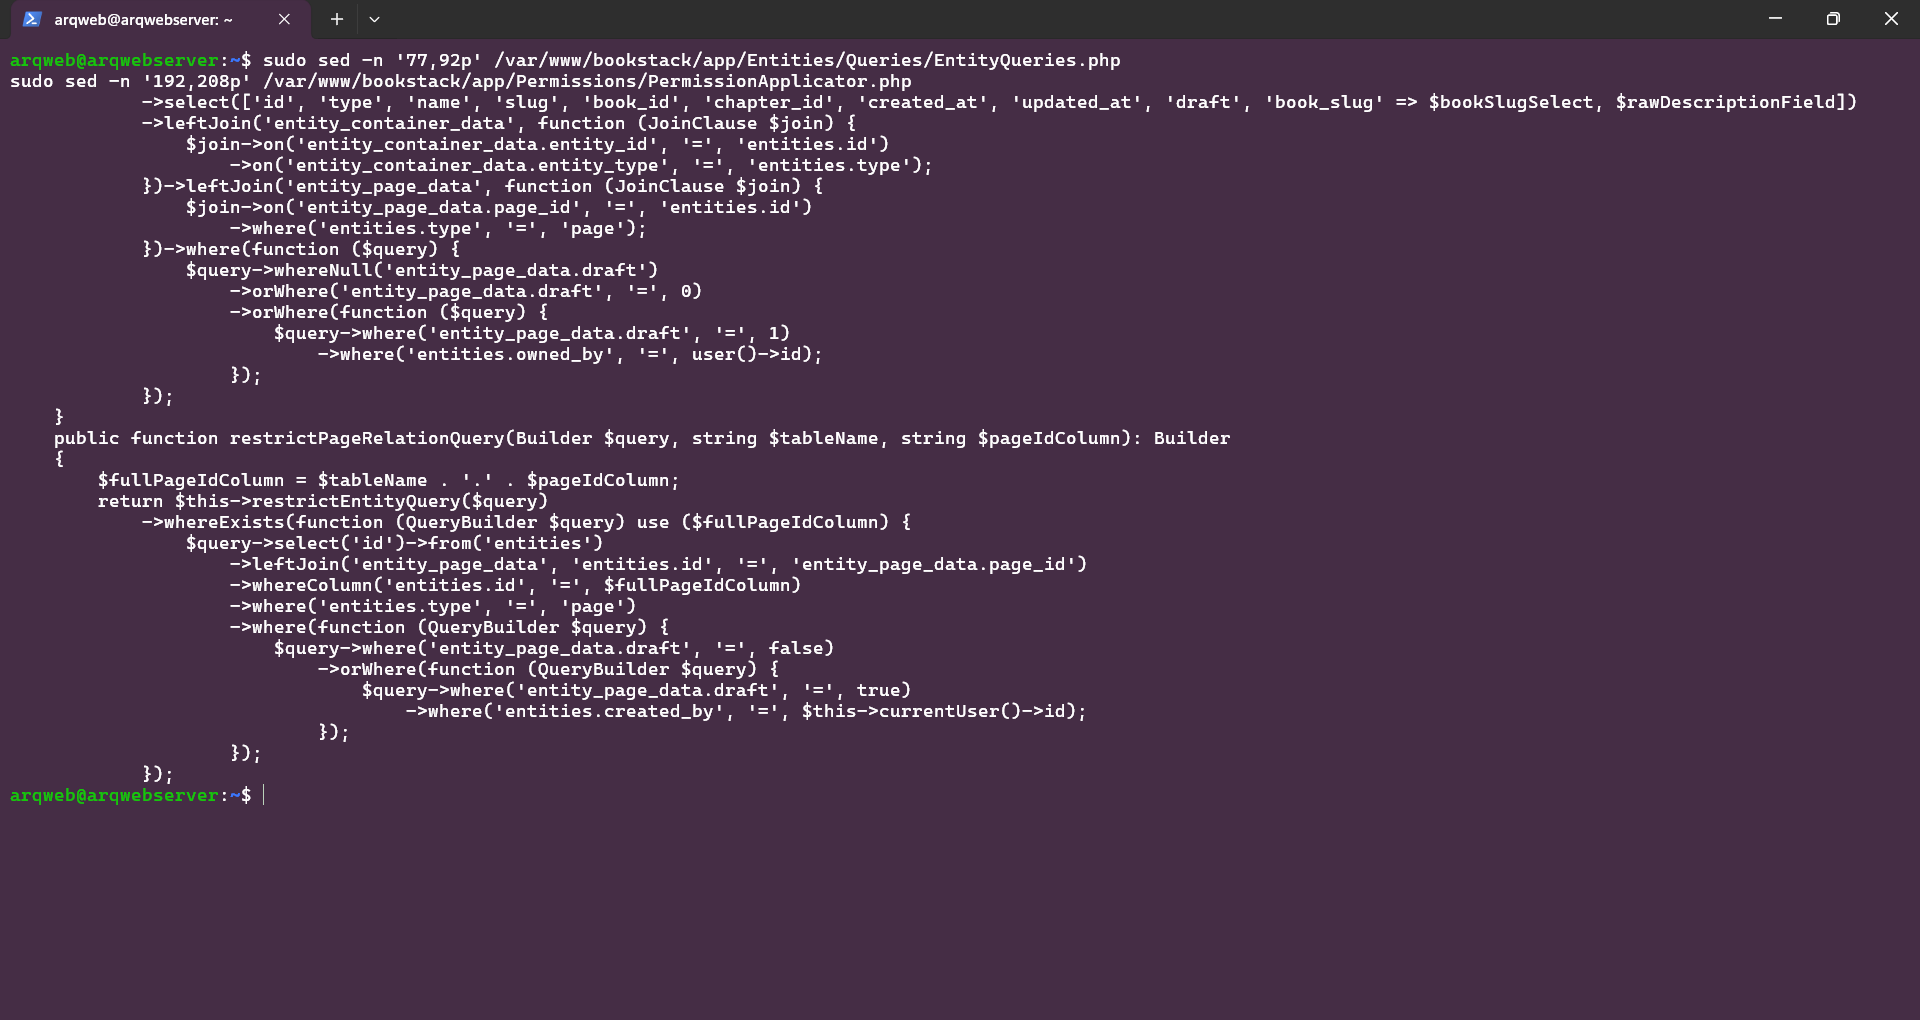
\includegraphics[width=\textwidth,height=0.64\textheight,keepaspectratio]{../../../cna/docs/evidencias/fase5/F5-E2-01-contenido-permisos.png}
\caption{Respaldo de F5-E2. Uniones compartidas de contenido y permisos, con filtros de borrador y propietario.}
\label{fig:f5-e2-contenido}
\end{figure}

\begin{figure}[H]
\centering
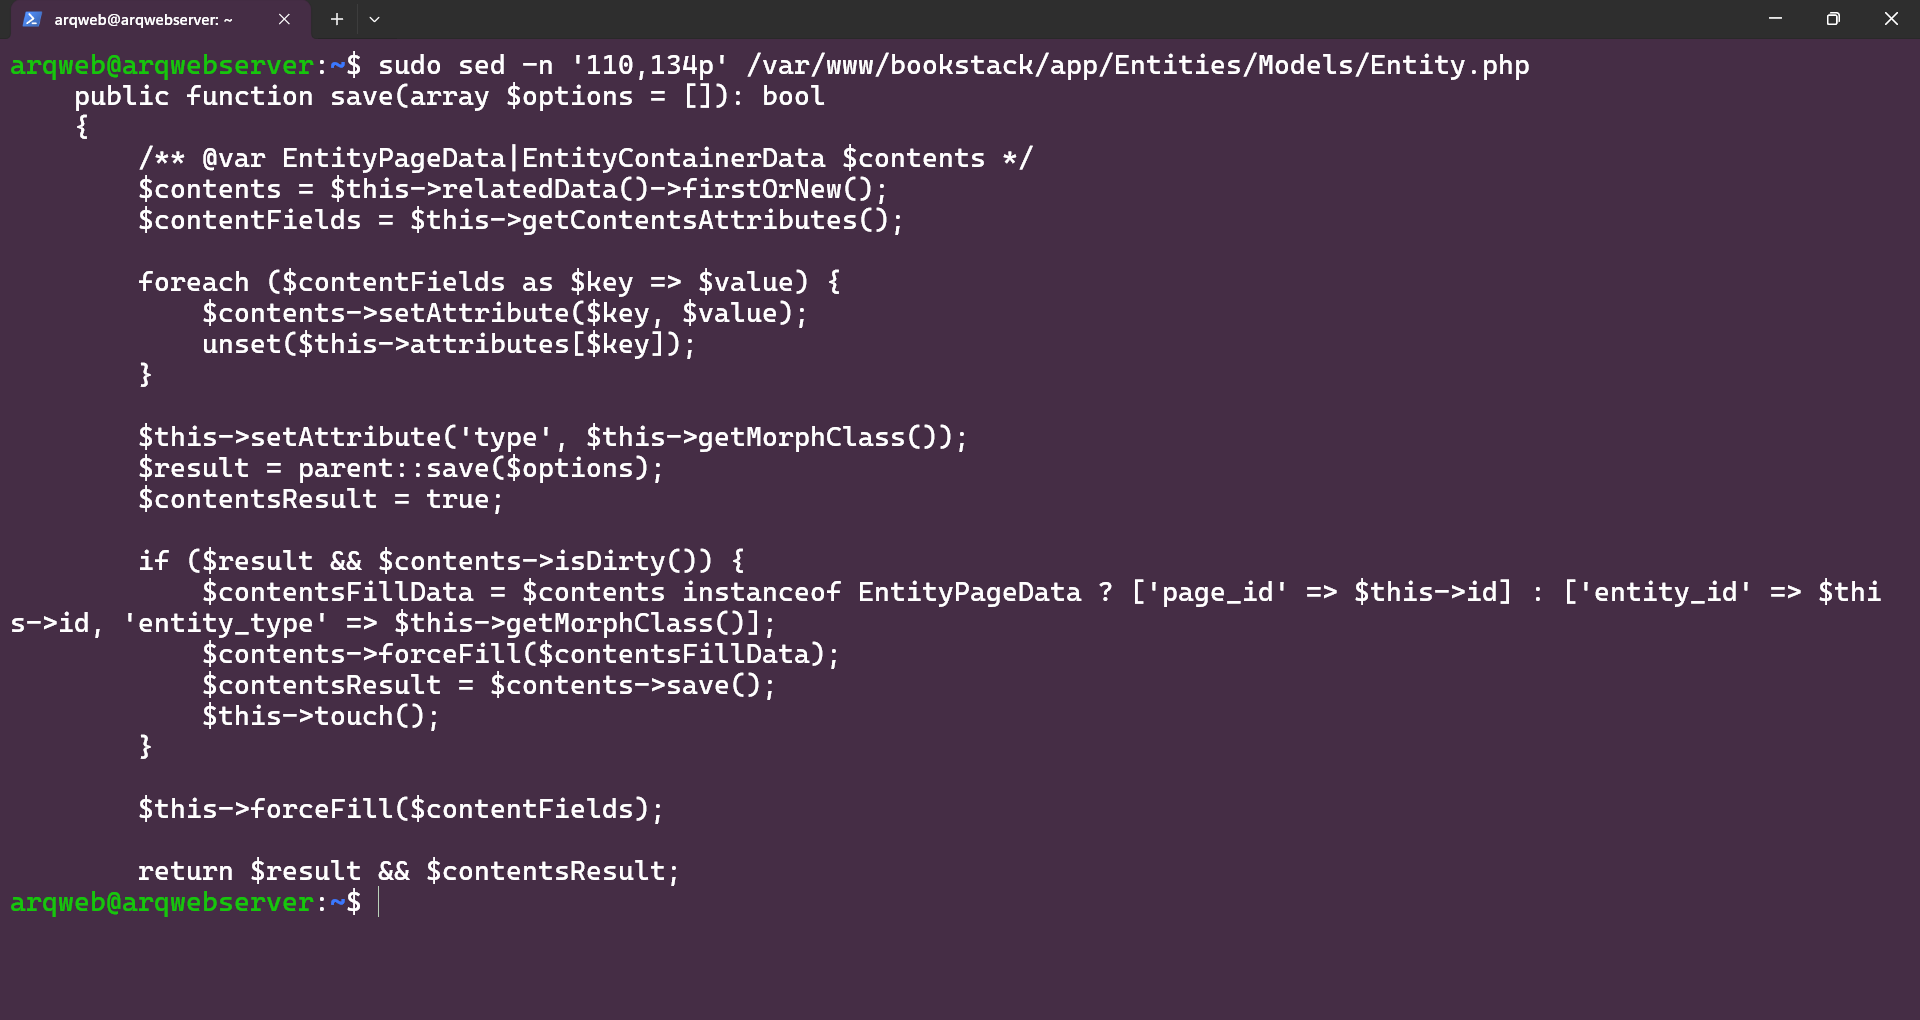
\includegraphics[width=\textwidth,height=0.64\textheight,keepaspectratio]{../../../cna/docs/evidencias/fase5/F5-E2-05-escritura-contenido.png}
\caption{Respaldo de F5-E2. Guardado de entidad y de sus datos específicos en el método Entity::save().}
\label{fig:f5-e2-escritura}
\end{figure}

\textbf{Búsqueda y actividad.} \texttt{SearchRunner} une los términos con
\texttt{entities} por ID y tipo. \texttt{SearchIndex} genera términos a partir
del nombre, el HTML o la descripción y las etiquetas, elimina el índice
previo e inserta los términos actualizados (R04).
\path{ActivityLogger::add()} guarda el registro de actividad antes de
llamar a \texttt{dispatchWebhooks()} (R05). Las
Figuras~\ref{fig:f5-e2-busqueda} y~\ref{fig:f5-e2-indice} respaldan las
consultas y escrituras identificadas.

\begin{figure}[H]
\centering
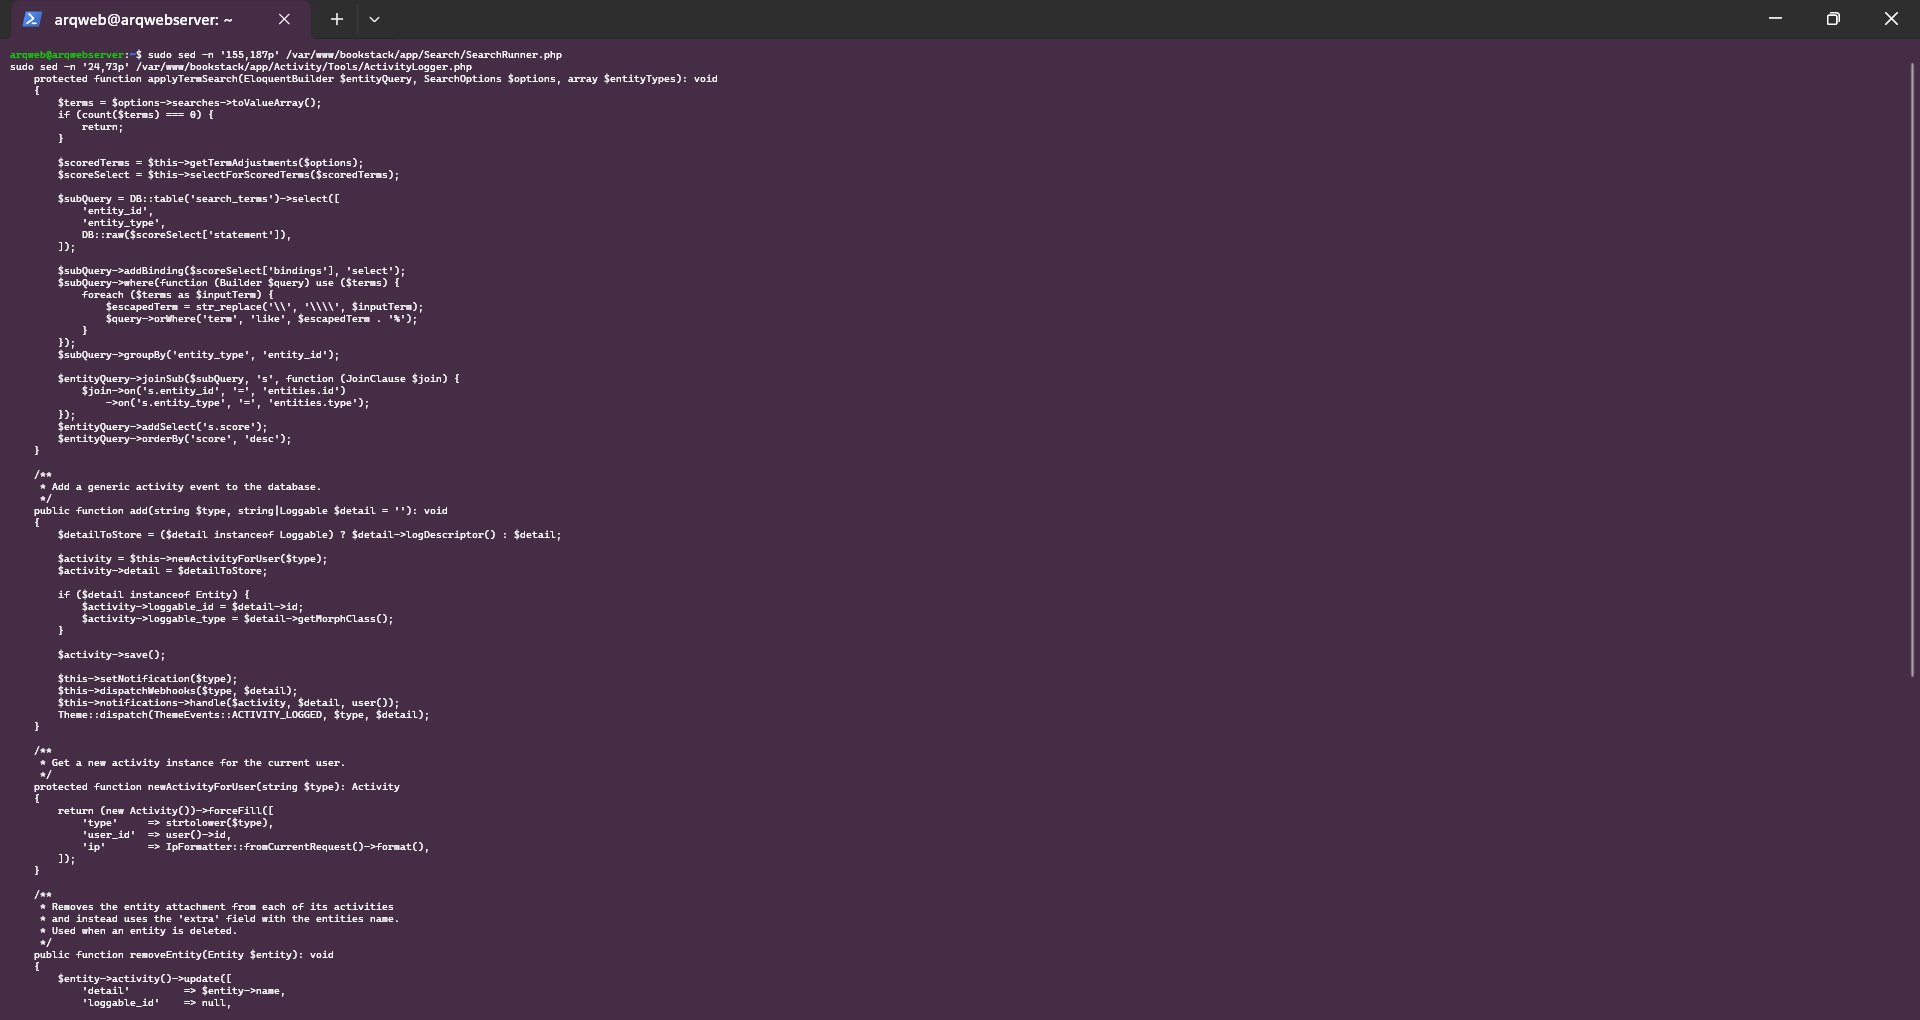
\includegraphics[width=\textwidth,height=0.64\textheight,keepaspectratio]{../../../cna/docs/evidencias/fase5/F5-E2-02-busqueda-auditoria.png}
\caption{Respaldo de F5-E2. Lectura del índice y persistencia de actividad con referencia al actor y al objeto.}
\label{fig:f5-e2-busqueda}
\end{figure}

\begin{figure}[H]
\centering
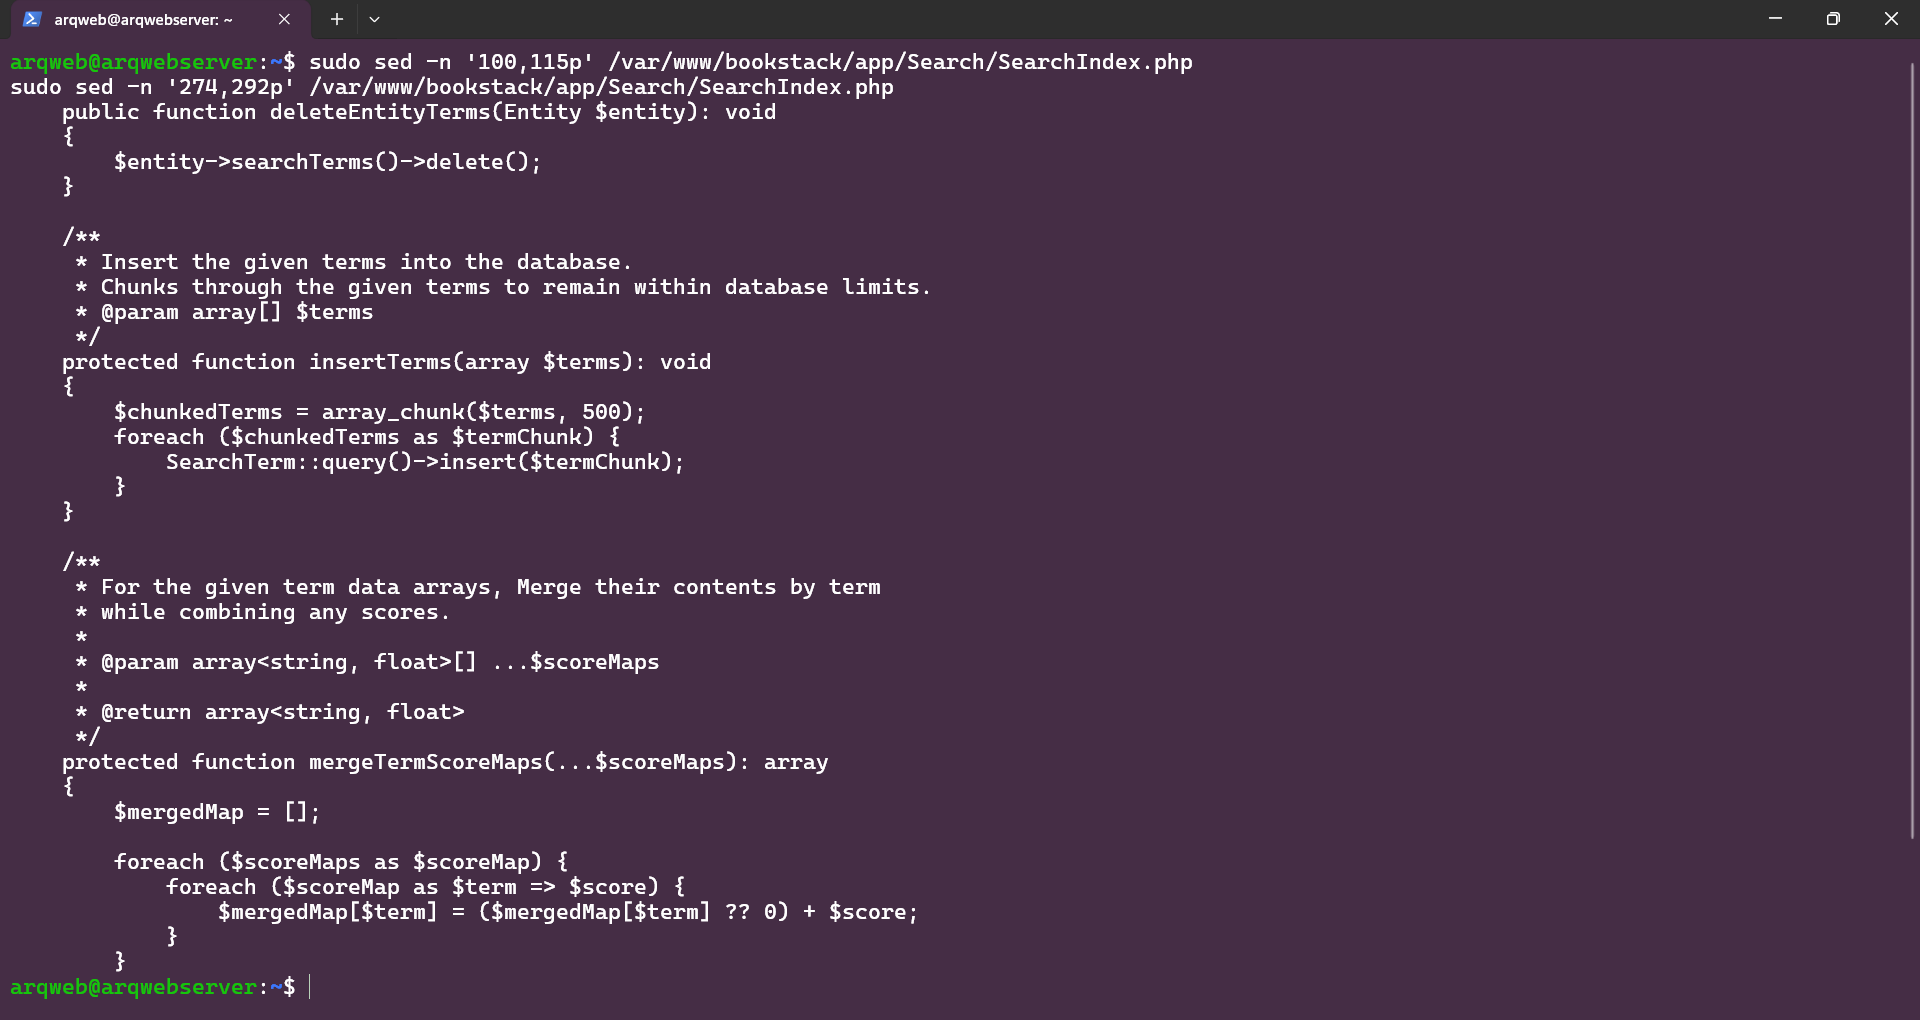
\includegraphics[width=\textwidth,height=0.64\textheight,keepaspectratio]{../../../cna/docs/evidencias/fase5/F5-E2-06-escritura-indice.png}
\caption{Respaldo de F5-E2. Eliminación de términos previos e inserción de los términos del índice de búsqueda.}
\label{fig:f5-e2-indice}
\end{figure}

\textbf{Imágenes y adjuntos.} \texttt{ImageService} guarda y elimina registros
y archivos; su limpieza de imágenes consulta el HTML de páginas y
revisiones para localizar referencias (R07,
Figura~\ref{fig:f5-e2-medios}). \texttt{AttachmentService} persiste los
metadatos de la subida, relaciona el archivo con la página por
\texttt{uploaded\_to} y coordina la baja del archivo y del registro
(R08, Figura~\ref{fig:f5-e2-adjuntos}). La visibilidad de los medios se
resuelve contra la página y sus permisos.

\begin{figure}[H]
\centering
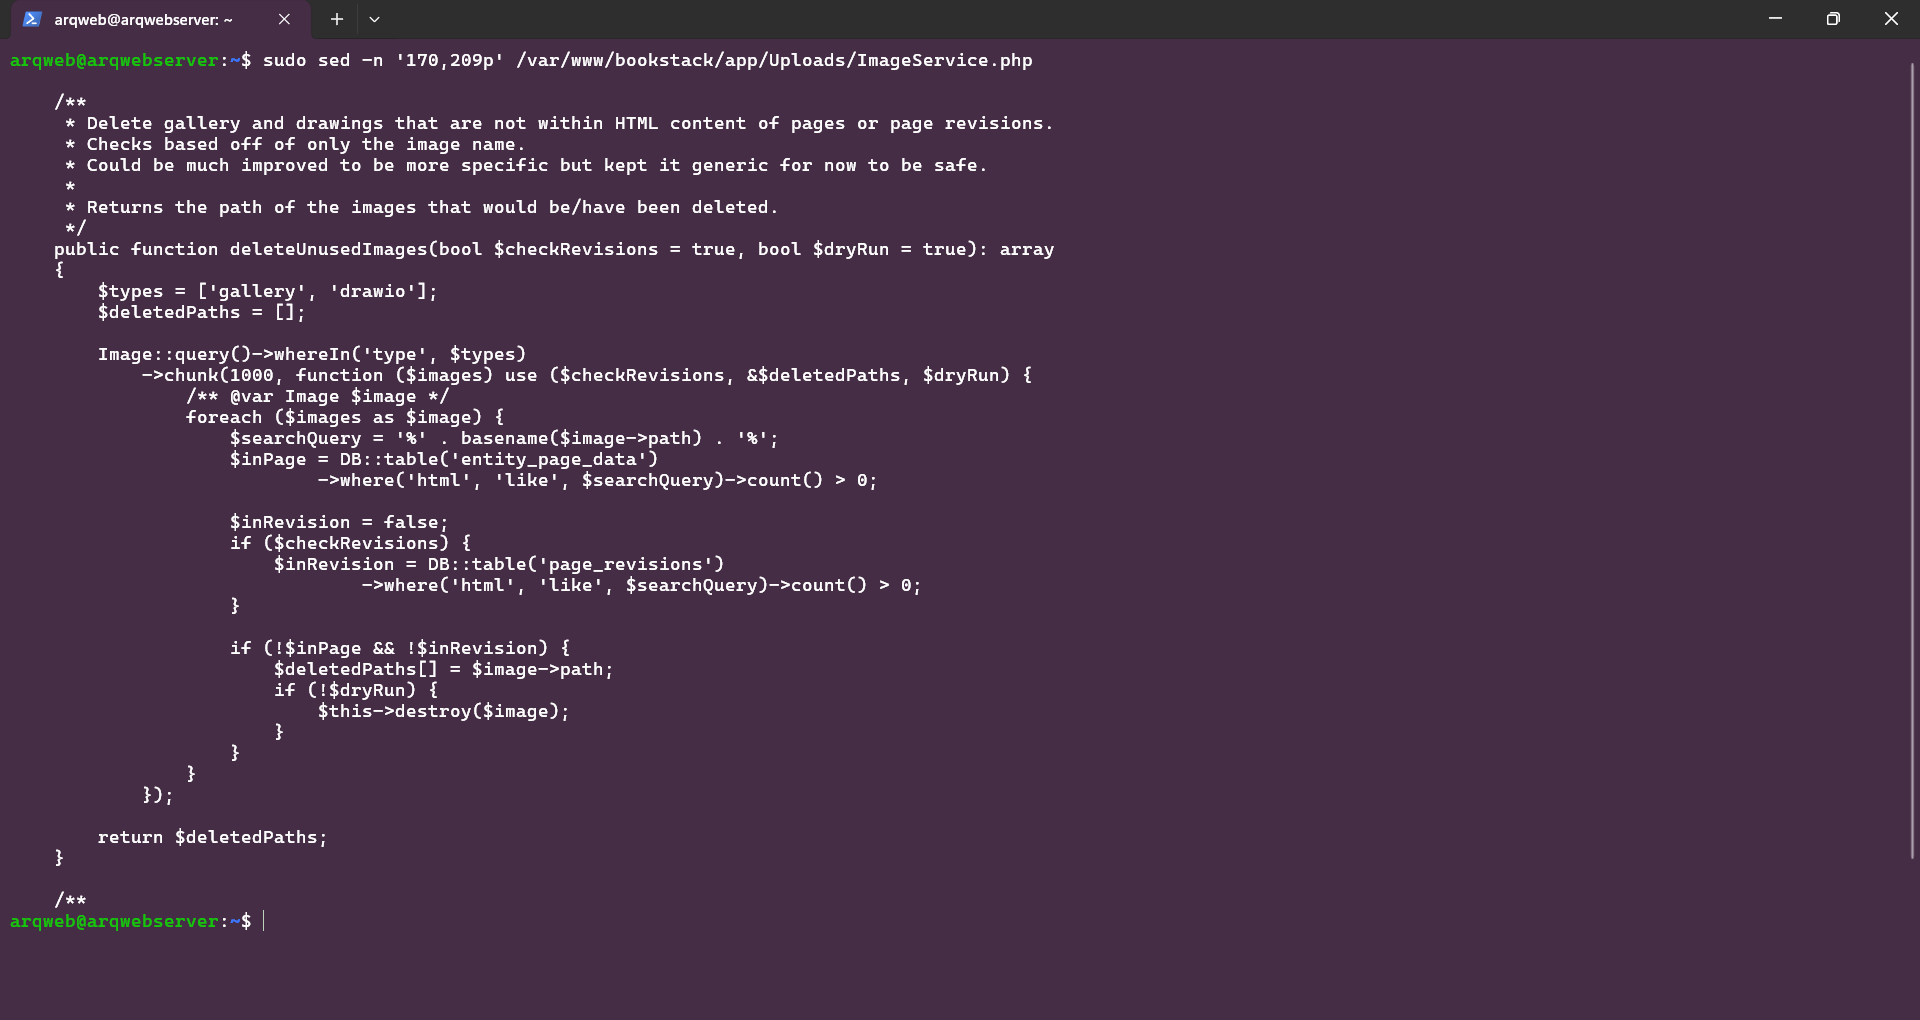
\includegraphics[width=\textwidth,height=0.64\textheight,keepaspectratio]{../../../cna/docs/evidencias/fase5/F5-E2-03-medios.png}
\caption{Respaldo de F5-E2. Dependencia de medios respecto del HTML actual e histórico para detectar imágenes sin uso.}
\label{fig:f5-e2-medios}
\end{figure}

\begin{figure}[H]
\centering
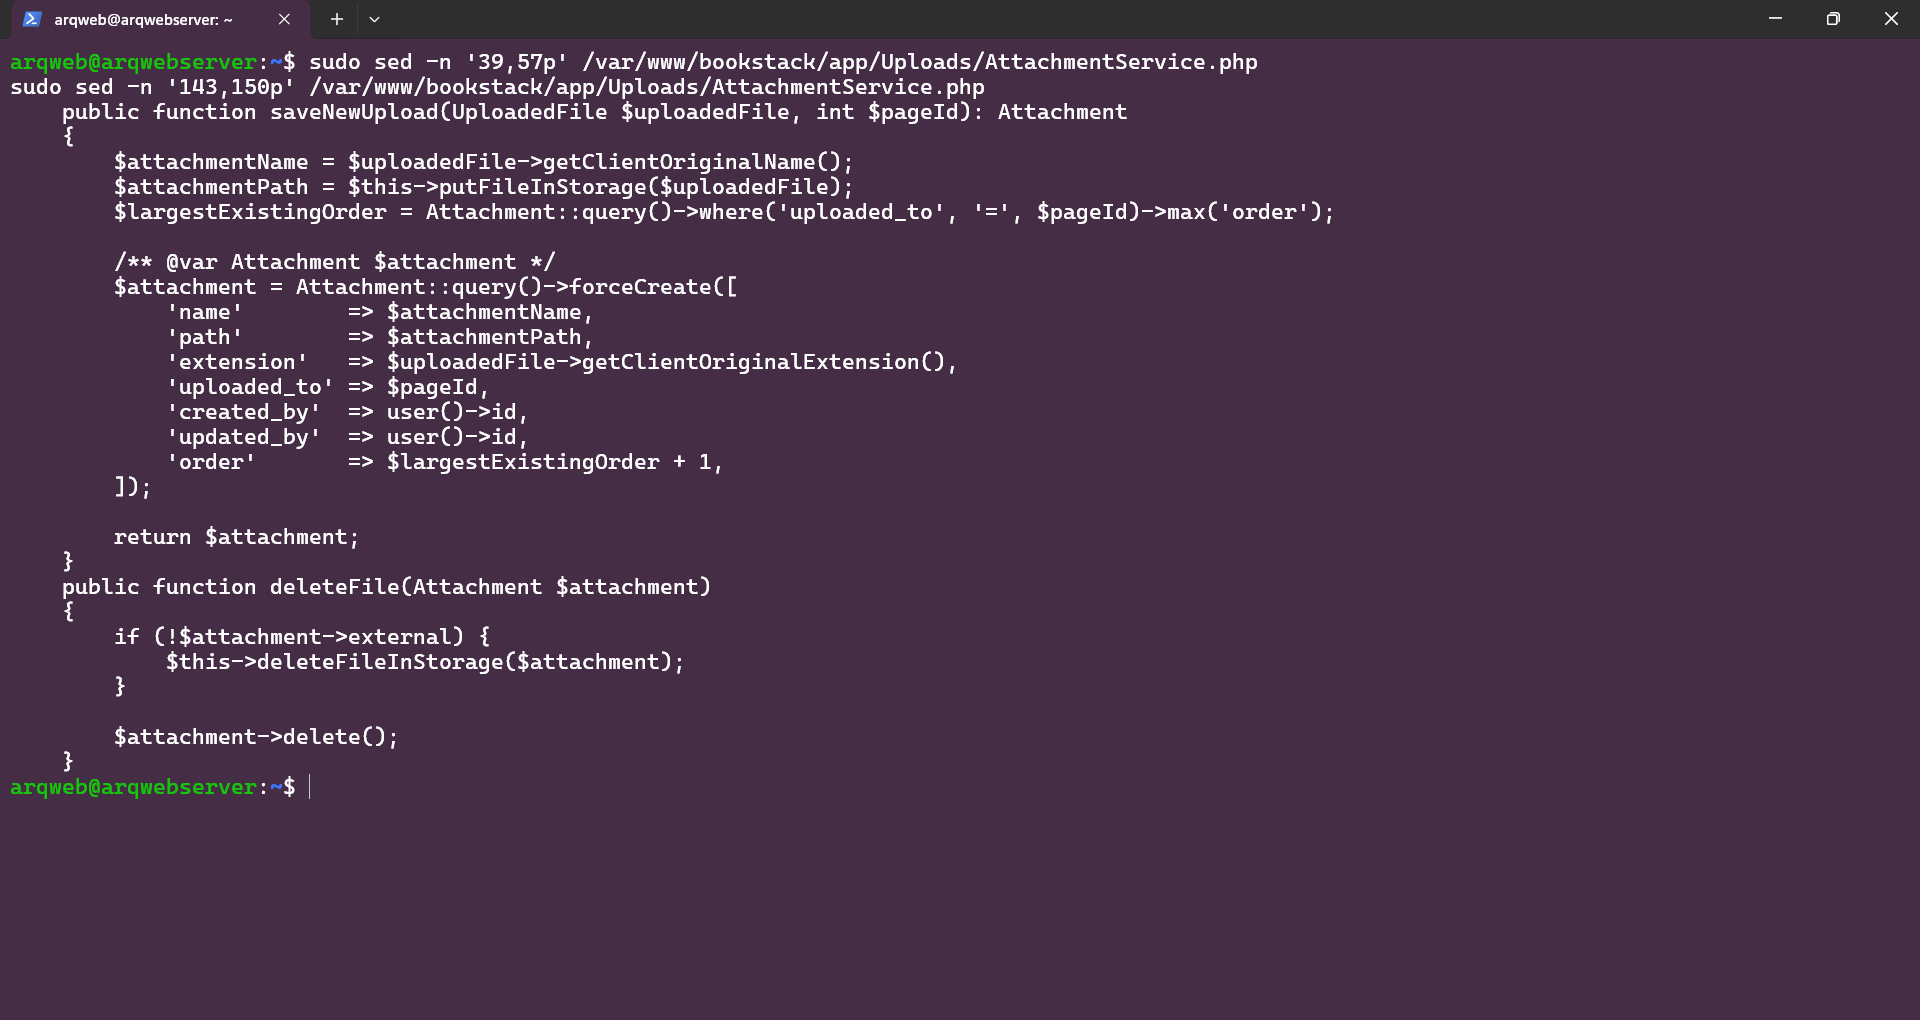
\includegraphics[width=\textwidth,height=0.64\textheight,keepaspectratio]{../../../cna/docs/evidencias/fase5/F5-E2-07-adjuntos.png}
\caption{Respaldo de F5-E2. Creación de metadatos de adjuntos y eliminación del archivo y su registro.}
\label{fig:f5-e2-adjuntos}
\end{figure}

\textbf{Usuarios, roles y permisos.} La consulta de permisos del usuario une
\texttt{role\_user}, \texttt{permission\_role} y \texttt{role\_permissions}.
\texttt{UserRepo} guarda cuentas y sincroniza roles
(Figura~\ref{fig:f5-e2-usuarios}). Al eliminar un usuario actualiza la autoría
en contenido, imágenes, adjuntos y revisiones, y reasigna la propiedad de
las entidades (Figura~\ref{fig:f5-e2-borrado}).
\texttt{PermissionsUpdater} modifica restricciones y
\path{JointPermissionBuilder} reconstruye \texttt{joint\_permissions}
(Figura~\ref{fig:f5-e2-permisos}). Estos recorridos explican el acceso
transversal a tablas administradas por otros módulos (R09--R10).

\begin{figure}[H]
\centering
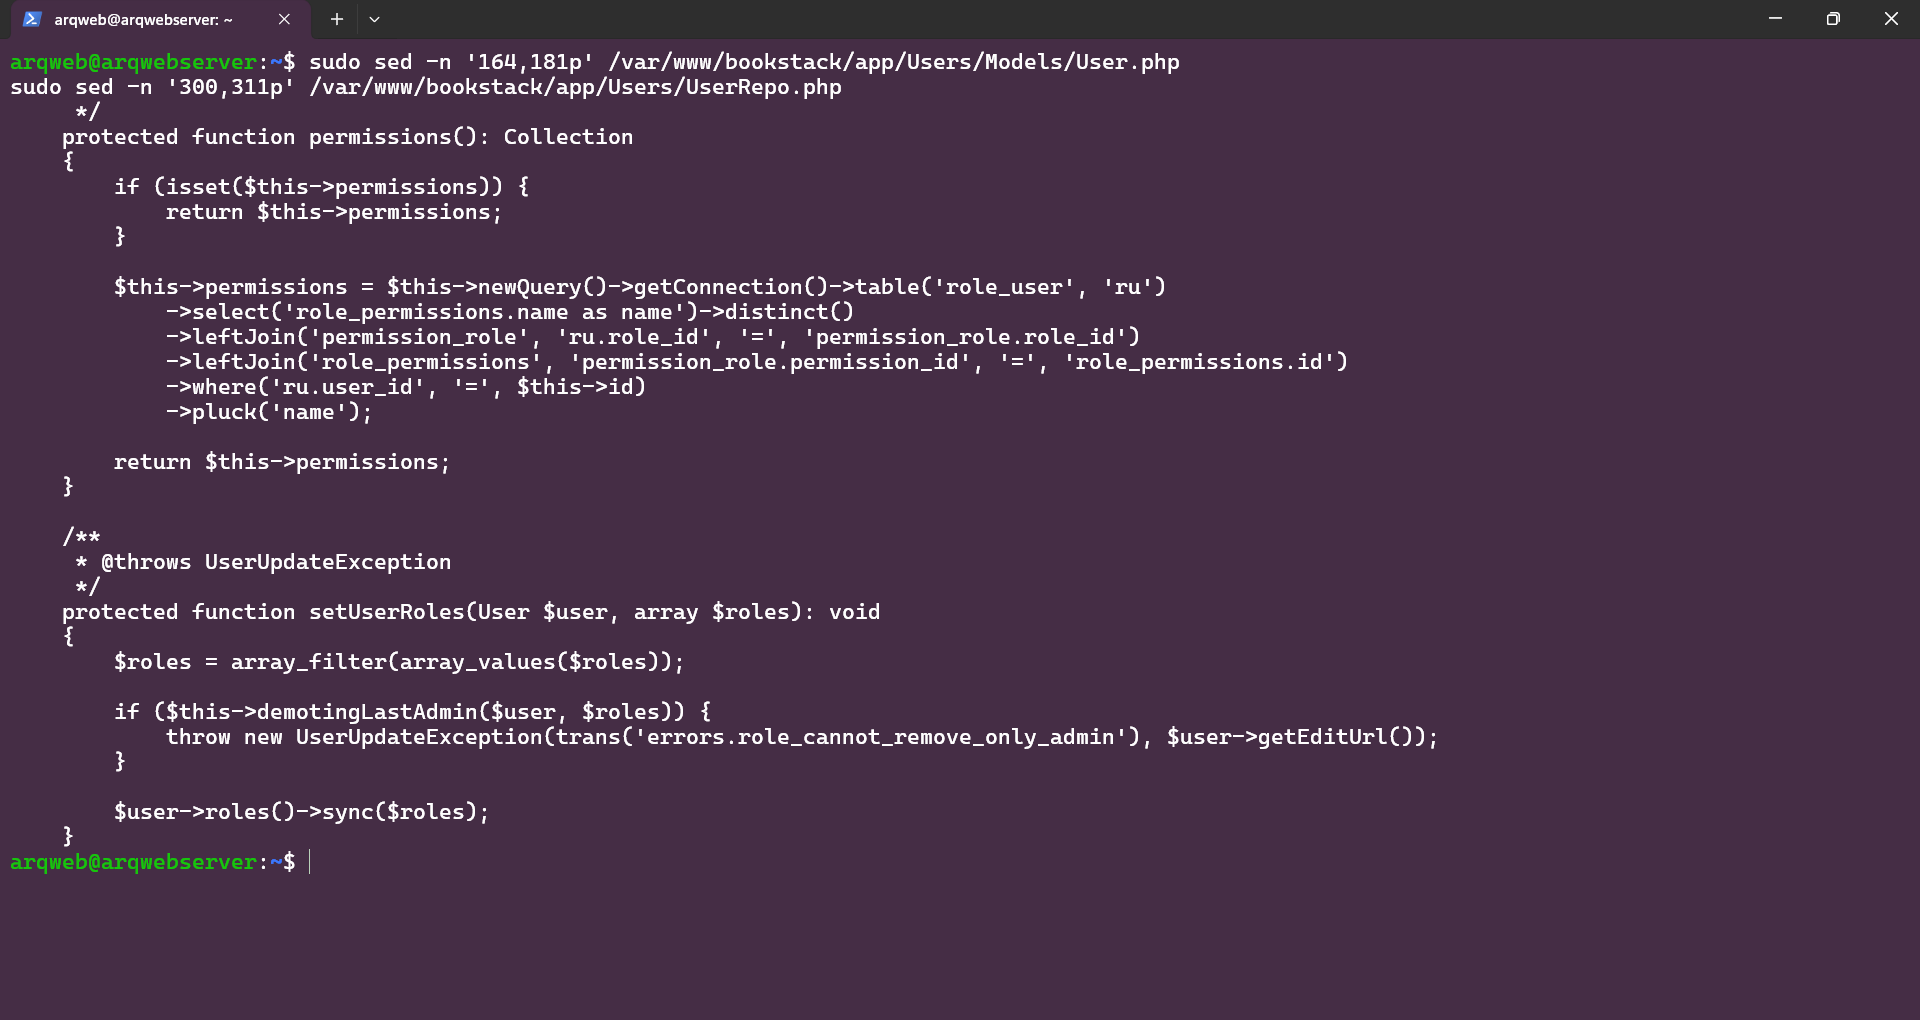
\includegraphics[width=\textwidth,height=0.64\textheight,keepaspectratio]{../../../cna/docs/evidencias/fase5/F5-E2-08-usuarios-roles.png}
\caption{Respaldo de F5-E2. Consulta de permisos del usuario y sincronización de su asignación de roles.}
\label{fig:f5-e2-usuarios}
\end{figure}

\begin{figure}[H]
\centering
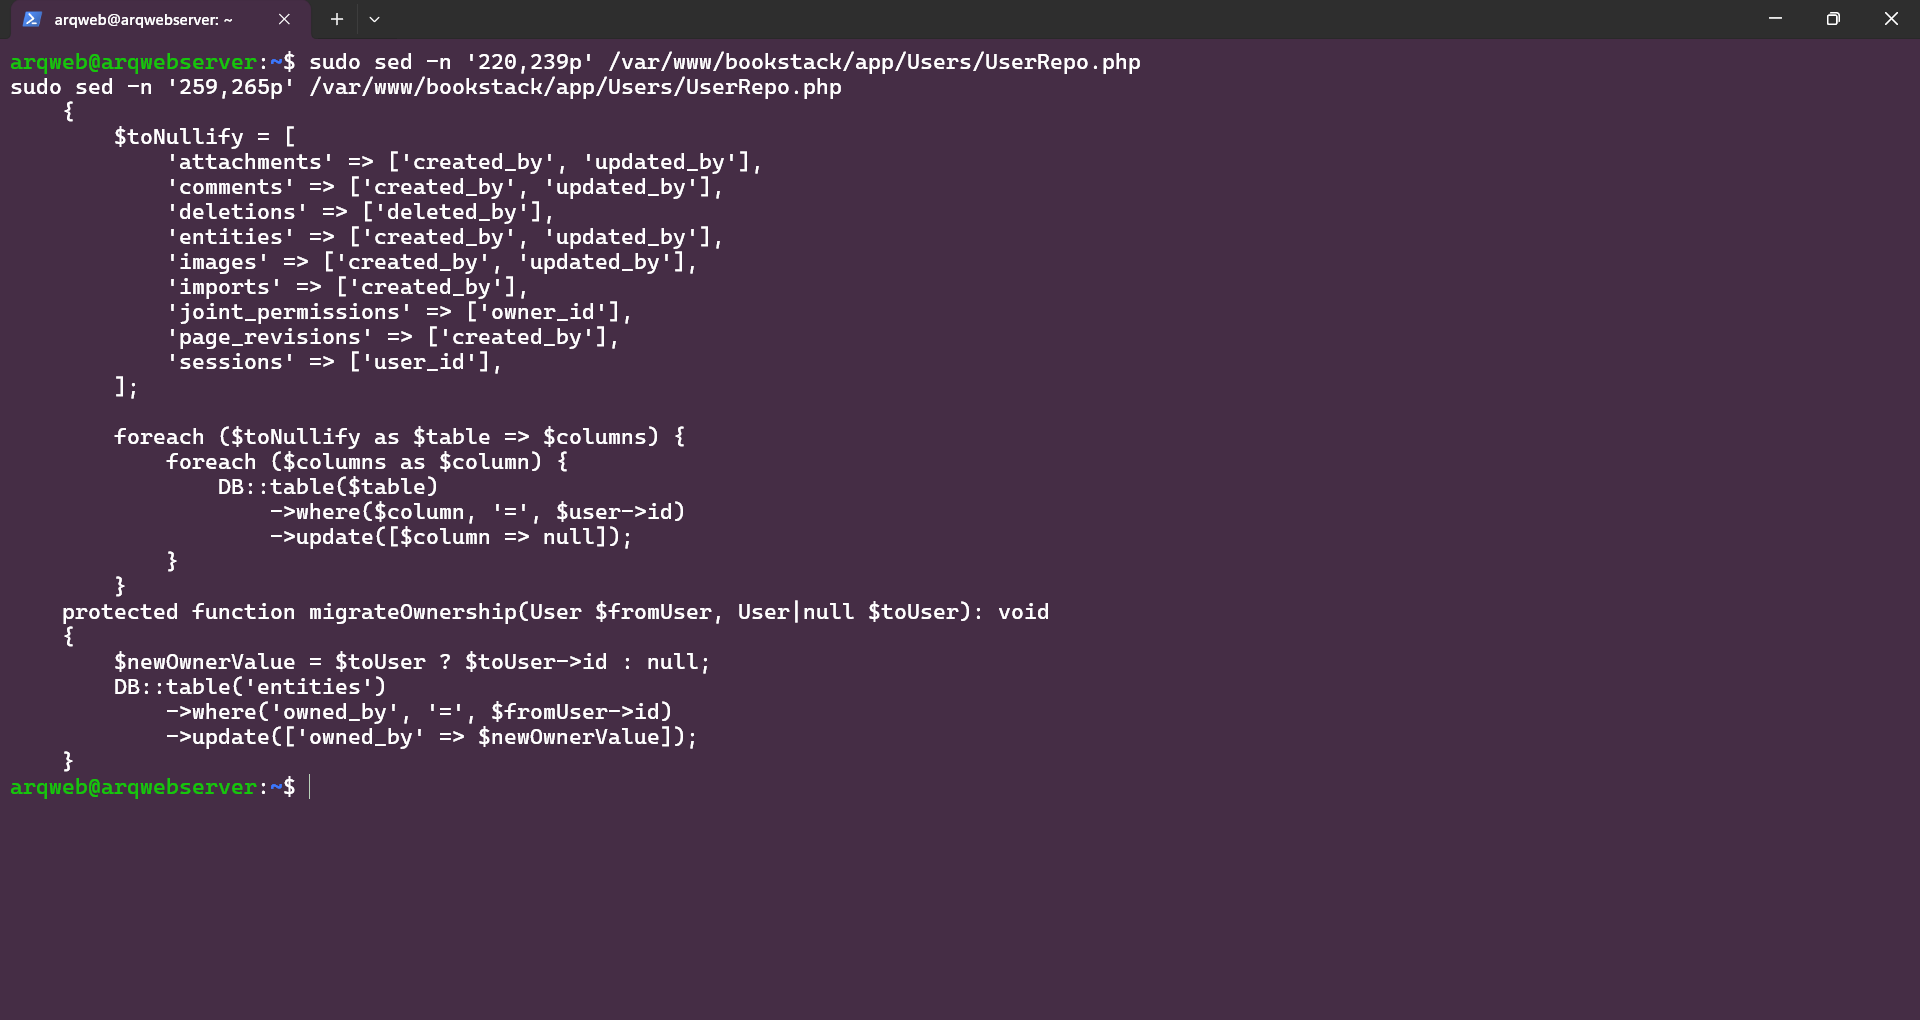
\includegraphics[width=\textwidth,height=0.64\textheight,keepaspectratio]{../../../cna/docs/evidencias/fase5/F5-E2-09-borrado-usuario.png}
\caption{Respaldo de F5-E2. Actualización de autoría y propiedad sobre tablas compartidas al eliminar una cuenta.}
\label{fig:f5-e2-borrado}
\end{figure}

\begin{figure}[H]
\centering
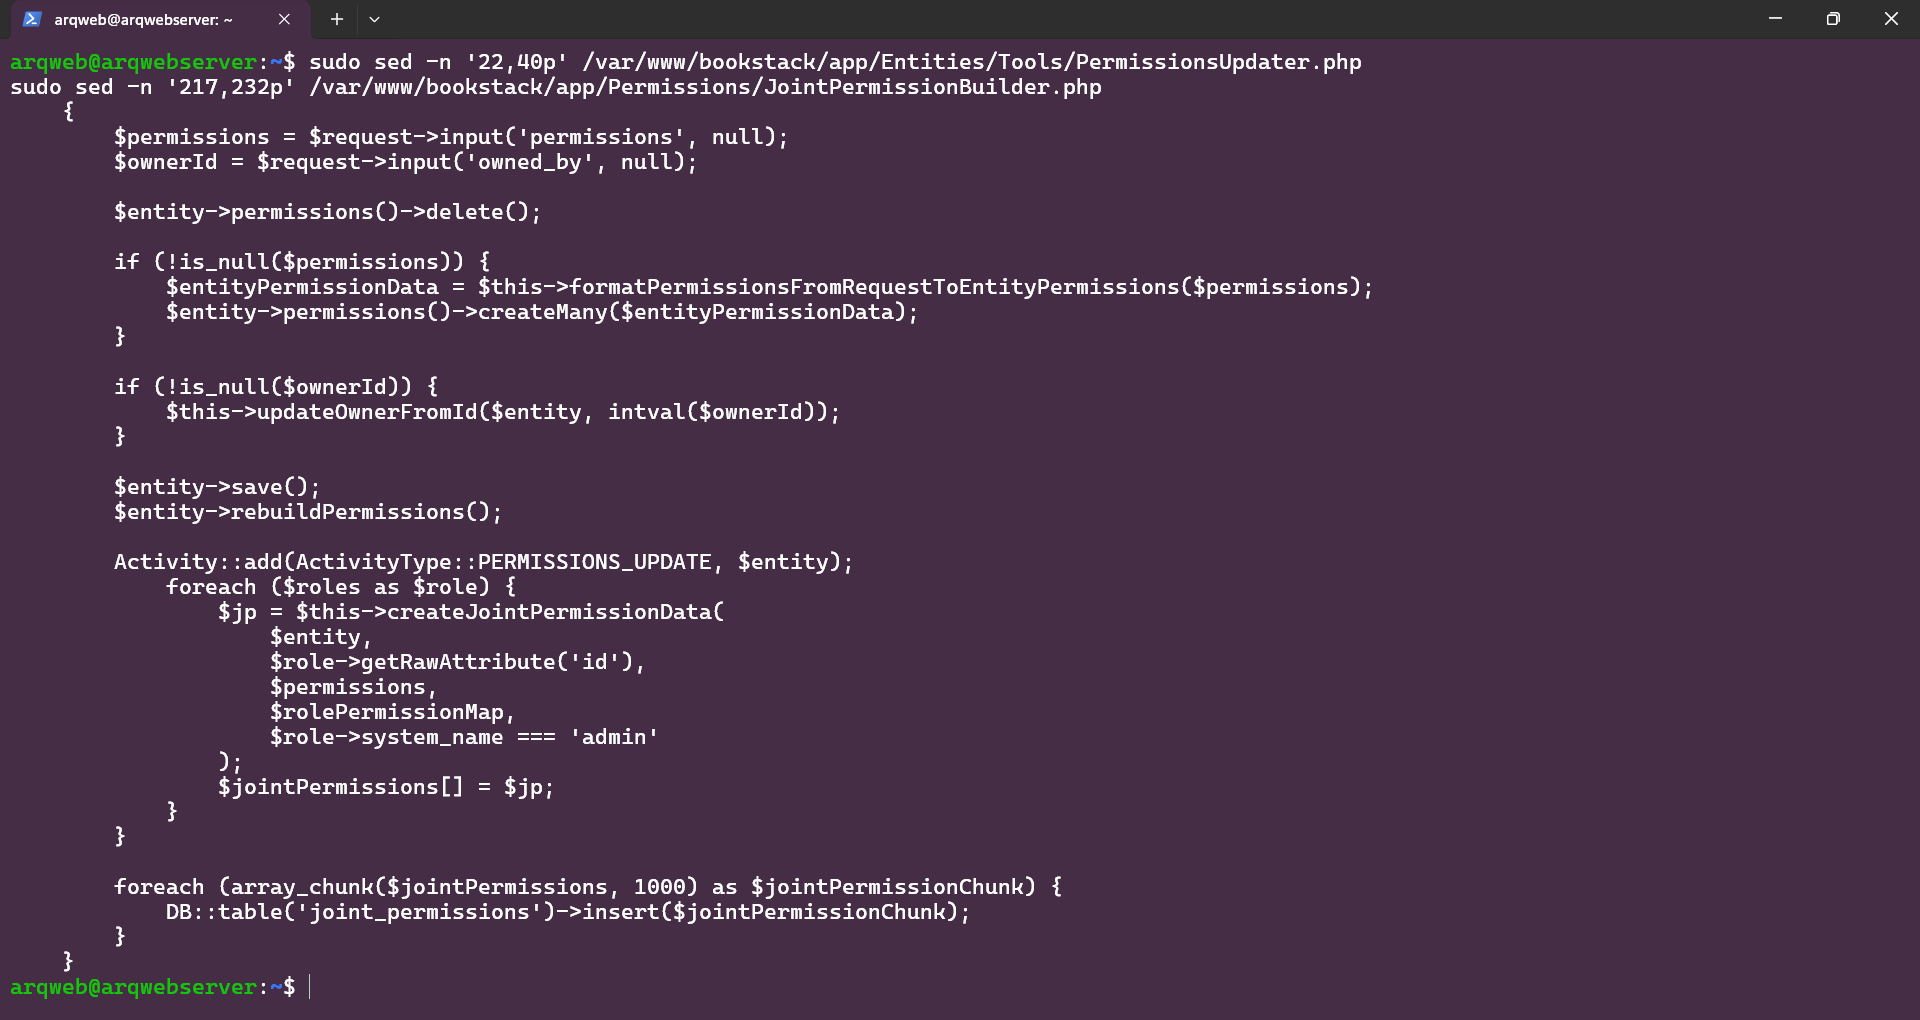
\includegraphics[width=\textwidth,height=0.64\textheight,keepaspectratio]{../../../cna/docs/evidencias/fase5/F5-E2-10-permisos-efectivos.png}
\caption{Respaldo de F5-E2. Persistencia de restricciones y reconstrucción de permisos efectivos.}
\label{fig:f5-e2-permisos}
\end{figure}

\textbf{Exportación.} Los controladores de API aplican el permiso
\texttt{ContentExport} y consultas visibles. El alcance de entidades une
los datos específicos; \texttt{BookContents} recupera el árbol de capítulos
y páginas. \texttt{ExportFormatter} obtiene Markdown o genera HTML para PDF
(R06, Figuras~\ref{fig:f5-e2-exporta} y~\ref{fig:f5-e2-exportb}). La ruta ZIP
lee etiquetas y adjuntos y recupera imágenes y archivos por sus modelos
(Figura~\ref{fig:f5-e2-zip}). La extracción debe conservar tanto la
visibilidad del contenido como el permiso de exportación.

\begin{figure}[H]
\centering
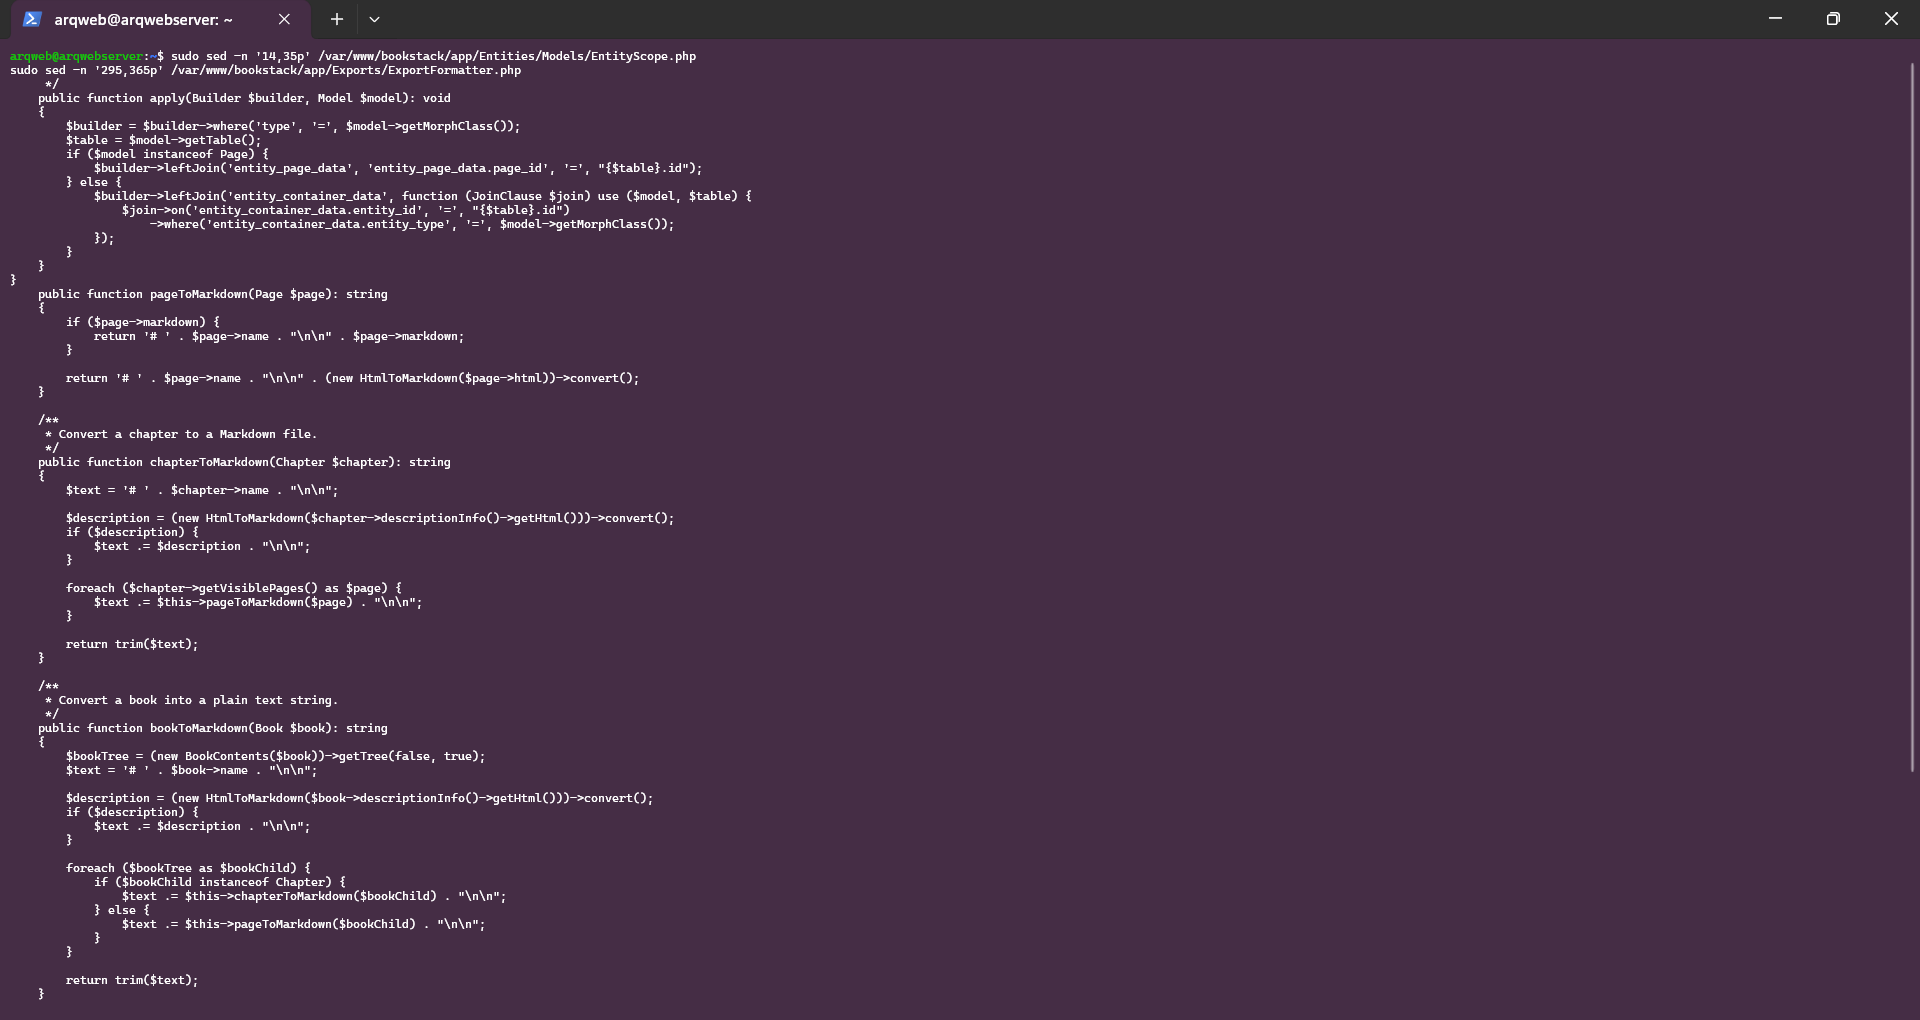
\includegraphics[width=\textwidth,height=0.64\textheight,keepaspectratio]{../../../cna/docs/evidencias/fase5/F5-E2-04-exportacion-markdown-a.png}
\caption{Respaldo de F5-E2. Alcance de entidades y conversión del contenido de página a Markdown.}
\label{fig:f5-e2-exporta}
\end{figure}

\begin{figure}[H]
\centering
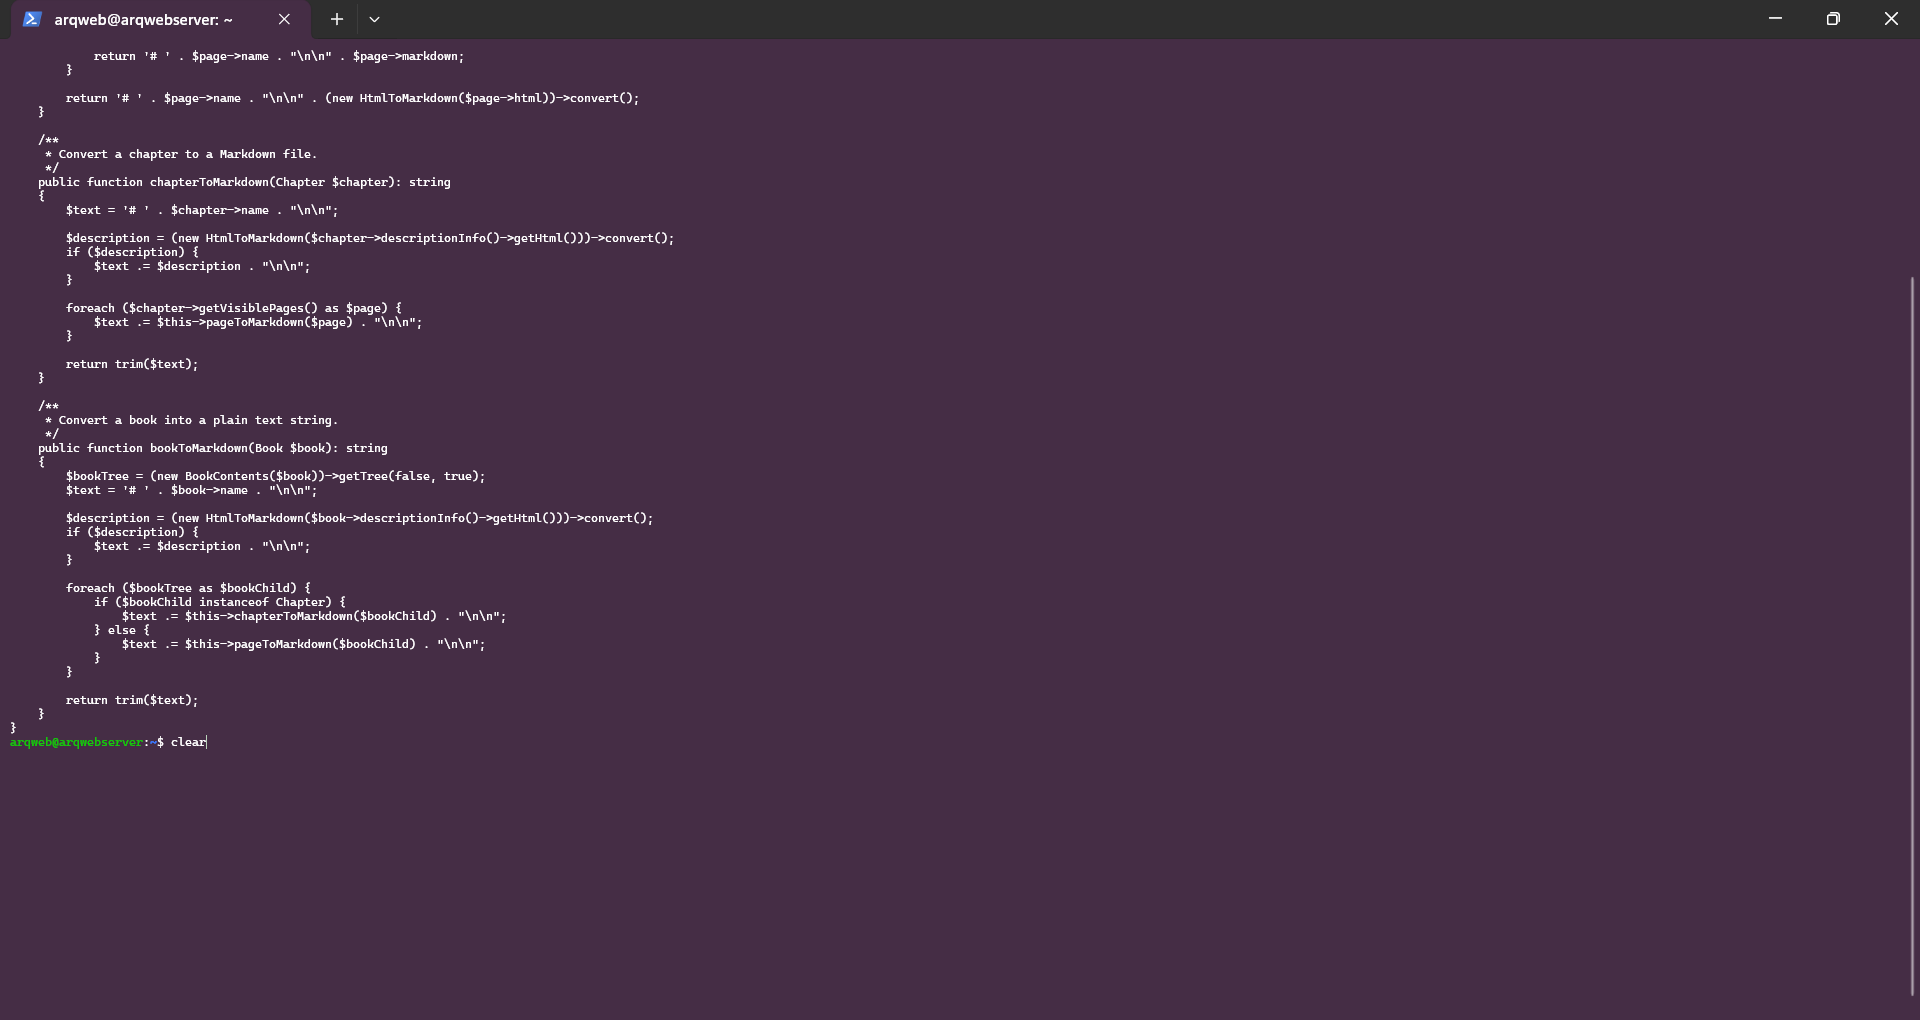
\includegraphics[width=\textwidth,height=0.64\textheight,keepaspectratio]{../../../cna/docs/evidencias/fase5/F5-E2-04-exportacion-markdown-b.png}
\caption{Respaldo de F5-E2. Recorrido de capítulos y páginas del libro durante la exportación Markdown.}
\label{fig:f5-e2-exportb}
\end{figure}

\begin{figure}[H]
\centering
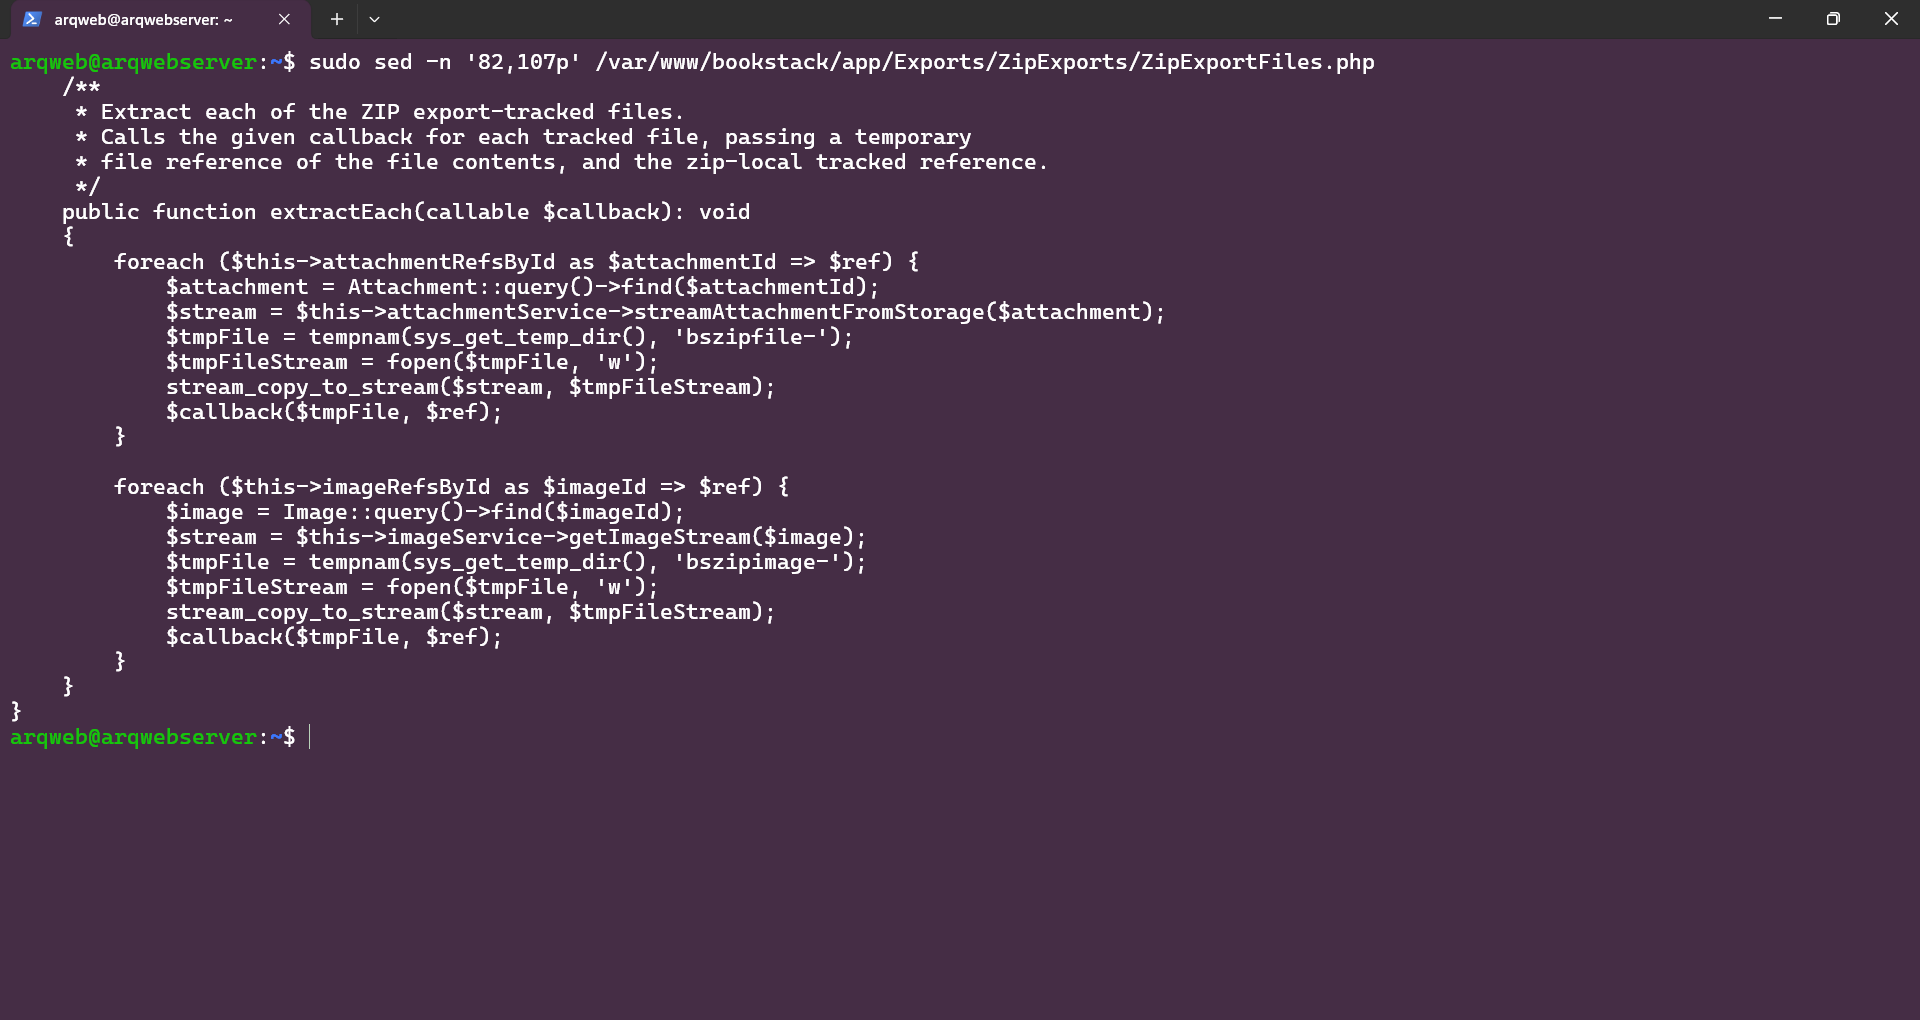
\includegraphics[width=\textwidth,height=0.64\textheight,keepaspectratio]{../../../cna/docs/evidencias/fase5/F5-E2-11-exportacion-archivos.png}
\caption{Respaldo de F5-E2. Lectura de adjuntos e imágenes para incorporar sus archivos a una exportación ZIP.}
\label{fig:f5-e2-zip}
\end{figure}

\subsubsection{Efecto de los acoplamientos sobre la extracción}
\begin{enumerate}[leftmargin=1.5em,itemsep=4pt]
\item \textbf{Contenido y búsqueda.} El guardado de contenido llama al indexador
local. La separación requiere un índice propio actualizado por eventos y
lecturas de API, con manejo de actualizaciones y borrados.
\item \textbf{Contenido y autorización.} La visibilidad depende de borradores,
propietario, roles y permisos efectivos. La consulta de datos mediante la
API y los resultados del nuevo servicio deben conservar ese alcance.
\item \textbf{Actividad y actores.} La auditoría registra acciones del contenido
y de la administración. La integración debe conservar actor, objeto, tipo
y momento de la acción mediante eventos normalizados.
\item \textbf{Medios y referencias.} La limpieza considera HTML y revisiones.
La gestión externa de archivos necesita preservar enlaces y referencias
para evitar eliminar recursos todavía utilizados.
\item \textbf{Exportación y contenido.} La exportación recorre entidades
visibles y puede incluir archivos. El servicio extraído consumirá la API
con autorización y administrará sus trabajos y artefactos propios.
\item \textbf{Usuarios y propiedad.} La eliminación de una cuenta actualiza
varias tablas. La representación de actores eliminados y la conservación
de sus referencias deben formar parte de los contratos de integración.
\end{enumerate}

\subsubsection{F5-E3: Mapa de contextos}
Se establecen seis contextos lógicos para analizar responsabilidades y
relaciones del dominio. La Figura~\ref{fig:f5-e3-contextos} representa su
situación actual dentro de BookStack. Las flechas indican información o
capacidad suministrada desde un proveedor hacia un consumidor. Los filtros
de autorización se aplican transversalmente en las consultas visibles.

\begin{figure}[H]
\centering
\begin{tikzpicture}[
ctx/.style={draw=NavyPrimary,fill=LightGrayBG,rounded corners=3pt,text width=3.5cm,minimum height=1.2cm,align=center,font=\small},
rel/.style={-{Stealth},thick,color=SlateSecondary},
lab/.style={font=\scriptsize,fill=white,inner sep=2pt,align=center}]
\node[ctx] (u) at (0,0) {Usuarios y permisos\\Proveedor de autorización};
\node[ctx] (c) at (0,-2.6) {Contenido\\Libros, capítulos y páginas};
\node[ctx] (m) at (-4.8,-2.6) {Imágenes y adjuntos\\Proveedor de archivos};
\node[ctx] (a) at (4.8,-2.6) {Actividad / auditoría\\Consumidor de acciones};
\node[ctx] (b) at (-2.5,-5.3) {Búsqueda\\Cliente de contenido};
\node[ctx] (x) at (2.5,-5.3) {Exportación\\Cliente de contenido};
\draw[rel] (u) -- node[lab,right]{Visibilidad y propiedad} (c);
\draw[rel] (m) -- node[lab,above]{Archivos} (c);
\draw[rel] (c) -- node[lab,above]{Acciones} (a);
\draw[rel] (c) -- node[lab,left]{Datos y etiquetas} (b);
\draw[rel] (c) -- node[lab,right]{Datos y árbol} (x);
\draw[rel] (u.east) -| node[lab,above,pos=0.3]{Acciones administrativas} (a.north);
\draw[rel] (c.north west) to[bend right=28] (m.north east);
\node[lab] at (-3.8,-1.1) {Referencias HTML\\y revisiones};
\end{tikzpicture}
\caption{F5-E3. Contextos lógicos del monolito y relaciones verificadas. Los seis contextos comparten el esquema de MariaDB; la matriz detalla sus accesos.}
\label{fig:f5-e3-contextos}
\end{figure}

\begin{samepage}
La relación de contenido con búsqueda y exportación se caracteriza como
\textit{cliente/proveedor}. Usuarios/permisos provee las reglas de acceso;
medios provee archivos y consulta referencias de contenido para su limpieza.
Actividad consume las acciones producidas por contenido y administración.
La persistencia compartida y las llamadas síncronas explican los límites
que deben adaptarse durante la extracción.
\end{samepage}

\begin{figure}[H]
\centering
\begin{tikzpicture}[
ctx/.style={draw=NavyPrimary,fill=LightGrayBG,rounded corners=3pt,text width=3.7cm,minimum height=1.1cm,align=center,font=\small},
acl/.style={ctx,draw=AccentBlue,fill=white},
rel/.style={-{Stealth},thick,color=SlateSecondary},
lab/.style={font=\scriptsize,fill=white,inner sep=2pt,align=center}]
\node[ctx,text width=7cm] (bs) at (0,0) {BookStack\\Contenido y autoridad de usuarios/permisos};
\node[acl] (http) at (-3.1,-2.2) {API REST\\Contenido autorizado};
\node[acl] (wh) at (3.1,-2.2) {Webhooks\\Acciones del monolito};
\node[acl] (ha) at (-3.1,-4.3) {ACL HTTP\\Adaptadores por servicio};
\node[acl] (ea) at (3.1,-4.3) {ACL de eventos\\event-bridge};
\node[ctx] (sx) at (-3.1,-6.6) {Búsqueda y exportación\\Clientes con datos propios};
\node[ctx] (ev) at (3.1,-6.6) {Canales de eventos\\Búsqueda y auditoría};
\draw[rel] (bs) -- (http);
\draw[rel] (bs) -- (wh);
\draw[rel] (http) -- (ha);
\draw[rel] (wh) -- (ea);
\draw[rel] (ha) -- node[lab,left]{Cliente/proveedor} (sx);
\draw[rel] (ea) -- node[lab,right]{Eventos normalizados} (ev);
\end{tikzpicture}
\caption{F5-E3. Límites de integración para la extracción. Las capas anticorrupción (ACL) adaptan la API y los Webhooks a contratos de los servicios consumidores.}
\label{fig:f5-e3-integracion}
\end{figure}

La ACL HTTP traduce las respuestas del monolito a las representaciones
propias de búsqueda y exportación. La ACL de eventos normaliza los Webhooks
antes de entregarlos a los consumidores. Medios constituye un contexto de
archivos y miniaturas con almacenamiento propio; su integración utiliza
URLs y API para conservar los recursos referenciados. El diseño de
contratos precisará el alcance de autorización y el ciclo de vida de los
archivos. La selección de herramientas y las decisiones de consistencia
se justifican en los ADR de A2.

Los fuentes editables del mapa se conservan en este archivo TikZ y en
\path{cna/docs/fase5-a1-contextos.mmd} y
\path{cna/docs/fase5-a1-contextos-propuesto.mmd}.

\subsubsection{Matriz de pruebas de A1 y resultado}
\begin{table}[H]
\centering\small
\begin{tabularx}{\textwidth}{p{1.3cm}p{1.8cm}Xp{2.3cm}}
\toprule
\textbf{Prueba} & \textbf{Evidencia} & \textbf{Resultado verificable} & \textbf{Estado} \\
\midrule
P26 & F5-E1 & Catálogo de 41 tablas y 280 columnas; cuatro FK; asignación de persistencia a los seis módulos. Tablas~\ref{tab:f5-modulos} y~\ref{tab:f5-fk}. & Completado \\
P27 & F5-E2 & Matriz de 6 módulos por 17 tablas principales, con accesos y dependencias delegadas respaldados por código. Tablas~\ref{tab:f5-matriz-1}--\ref{tab:f5-matriz-3}. & Completado \\
P28 & F5-E3 & Mapa de contextos, relaciones cliente/proveedor y capas anticorrupción. Figuras~\ref{fig:f5-e3-contextos} y~\ref{fig:f5-e3-integracion}. & Completado \\
\bottomrule
\end{tabularx}
\caption{Continuación de la matriz consolidada para A1, desde P26.}
\label{tab:f5-pruebas}
\end{table}

A1 establece el inventario de los seis módulos, su acoplamiento sobre tablas
compartidas y los límites de contexto para la extracción. La matriz vincula
las lecturas y escrituras con el código instalado y el mapa define las
relaciones funcionales y de integración que servirán de base a los ADR.


\endgroup
